\documentclass[12pt]{article}
\usepackage[a4paper,margin=1in]{geometry}
\usepackage{setspace}
\usepackage{graphicx}
\usepackage{amsmath}
\usepackage{siunitx}
\usepackage{booktabs}
\usepackage{caption}
\usepackage{url}
\usepackage{float}
\usepackage{xcolor}

% --- helpers ---
\doublespacing
\setlength{\parskip}{0.8em}
\newcommand{\TODO}[1]{\textbf{\color{red}{[TODO: #1]}}}

\begin{document}

\begin{center}
\textbf{\Large Verifying the First Law of Thermodynamics in a Pressurized Tank: Heat Loss, Work, and Internal Energy} \\[0.5em]
Kevin Peng (1011043238), Boya Zhang (1010855638), Yang Yang Zhang (1011437786)\\[0.5em]
CHE260 PRA 0101 \\
First Law of Thermodynamics Lab \\
October 15th, 2025 \\
\end{center}

\section*{Abstract}
This experiment verified the First Law of Thermodynamics by measuring heat loss, work input, and internal energy changes in a pressurized air tank. Four trials were conducted at constant pressure (40--80 psig) and temperature (40--60°C) with air continuously added. At steady state, the total heat loss rate ranged from $\dot{Q}_{\text{total}} = 95 \pm 1$ W (Trial A) to $240 \pm 0.2$ W (Trial D), of which $14 \pm 1$--$32 \pm 3$ W was conducted through acrylic walls and the remainder through aluminum plates. The constant-volume specific heat was estimated as $c_v = 63$--$82~\mathrm{kJ/(kg \cdot K)}$, and propeller work input ($\sim 0.7$ W) was negligible compared to heat loss. Steady-state energy balance from heater power vs.\ losses was consistent within fit uncertainty; transient $c_v$ estimates were systematically high due to small $\Delta T$ and model assumptions.

\section*{Introduction}
The First Law of Thermodynamics expresses the principle of energy conservation, stating that energy cannot be created or destroyed but only transformed between heat, work, and internal energy \cite{che260_manual}. For a control volume at steady state with entering/leaving mass, this relationship is $\dot{Q} - \dot{W} = \dot{m}(h_{\text{out}} - h_{\text{in}})$, where $\dot{Q}$ is heat transfer rate and $\dot{W}$ is work.

The experiment aims to:
\begin{enumerate}
    \item Determine the mass of air added to a rigid tank using ideal gas law and absolute pressure measurements.
    \item Measure steady-state heat loss rate by fitting a linear trend to cumulative heater energy, and decompose it into wall conduction (cylindrical) and plate losses (residual).
    \item Estimate constant-volume specific heat capacity $c_v$ from controlled heating segments and calculate propeller work using fan similarity laws.
\end{enumerate}

Key equations applied: Ideal gas law ($PV=nRT$), cylindrical conduction ($\dot{Q}=\frac{2k\pi L\,\Delta T}{\ln(r_2/r_1)}$), and propeller power scaling ($P_2 = P_1 \frac{\rho_2}{\rho_1} \left(\frac{n_2}{n_1}\right)^3 \left(\frac{D_2}{D_1}\right)^5$).

\section*{Experimental Method}
Two rigid acrylic tanks with pressure transducers, thermocouples, a mass-flow controller, and two PID heaters are operated via LabVIEW. Four trials: 40~psig \& 40\si{\celsius} (A), 80~psig \& 40\si{\celsius} (B), 40~psig \& 60\si{\celsius} (C), 70~psig \& 60\si{\celsius} (D) \cite{che260_manual}. At steady state, LabVIEW logs temperature, pressure, and cumulative heater energy.

\begin{figure}[H]
    \centering
    \includegraphics[width=0.8\textwidth]{graphs/apparatus.png}
    \caption{Schematic of tank, sensors, heaters, and data acquisition.}
    \label{fig:apparatus}
\end{figure}

The apparatus consists of a rigid tank with internal volume $\approx 0.04$ m$^3$, fitted with a 1 kW electric heater (on/off relay control to maintain setpoint $\pm 0.5$ K), a propeller fan (1725 rpm, 1 hp motor), and a data acquisition system. Key sensors include: absolute pressure transducers (psig output converted to psia), RTD temperature probes (gas interior, wall exterior, ambient), and an energy meter (watts). 

\textbf{Part 1:} A regulated mass of air (from a pressurized source) was admitted into the tank via a mass-flow rotameter, and the cumulative mass was integrated from the volumetric flow rate. Initial and final pressures/temperatures were recorded to apply the ideal gas law: $m_{\text{left}} = m_{\text{added}} \times [1 + 1/(P_2 T_1 / (P_1 T_2) - 1)]$.

\textbf{Part 2:} The tank was heated to four setpoint temperatures (40, 40, 59, 59 \textdegree C across trials A–D); once at steady state ($\pm 0.5$ K for 5 min), the cumulative heater energy and temperature were logged at 1-second intervals. A linear fit to the energy data yielded the heat loss rate $\dot{Q}_{\text{total}}$. Acrylic-wall conduction was calculated from cylindrical geometry and temperature difference; plate losses were inferred as the residual.

\textbf{Part 3:} A 24-second heating transient (rising from 60 K below setpoint to near setpoint) was selected for $c_v$ calculation. Heater energy, tank mass, and temperature rise were used to back-calculate $c_v$. The propeller fan ran at constant speed (1725 rpm) throughout, and its power input was estimated using manufacturer similarity laws.

\section*{Results and Discussion}

\subsection*{Part 1 — Mass in the Left Tank}
\begin{table}[H]\centering
\caption{Part 1 summary: Pressures converted from psig to psia using measured atmospheric pressure. Ratios $P_2T_1/(P_1T_2)$ confirm ideal gas behavior.}
\label{tab:part1}
\begin{tabular}{@{}lccccccc@{}}
\toprule
Trial & $P_{\text{init,abs}}$ (psia) & $T_{\text{init}}$ (\si{\celsius}) & $P_{\text{final,abs}}$ (psia) & $T_{\text{final}}$ (\si{\celsius}) & $m_{\text{added}}$ (kg) & $m_{\text{left}}$ (kg) & Ratio $\frac{P_2T_1}{P_1T_2}$ \\
\midrule
A & 15.48 & 25.3 & 54.40 & 28.8 & 0.0296 & 0.0415 & 3.47 \\
B & 15.39 & 27.1 & 94.62 & 29.7 & 0.0600 & 0.0718 & 6.10 \\
C & 16.58 & 33.6 & 55.07 & 33.7 & 0.0287 & 0.0411 & 3.32 \\
D & 16.21 & 37.9 & 83.91 & 36.0 & 0.0513 & 0.0634 & 5.21 \\
\bottomrule
\end{tabular}
\end{table}

\paragraph{Discussion.} All trials showed small temperature increases (2–4 \textdegree C) despite large pressure ratios (3.3–6.1×), consistent with adiabatic compression of added gas. The pressure-ratio test validates the ideal gas law assumption and the absolute pressure measurement technique. The net difference $(m_{\text{added}} - m_{\text{left}})$ was approximately $-12$ g, representing an instrumentation bias in the filling/sealing procedure.

\begin{figure}[H]
\centering
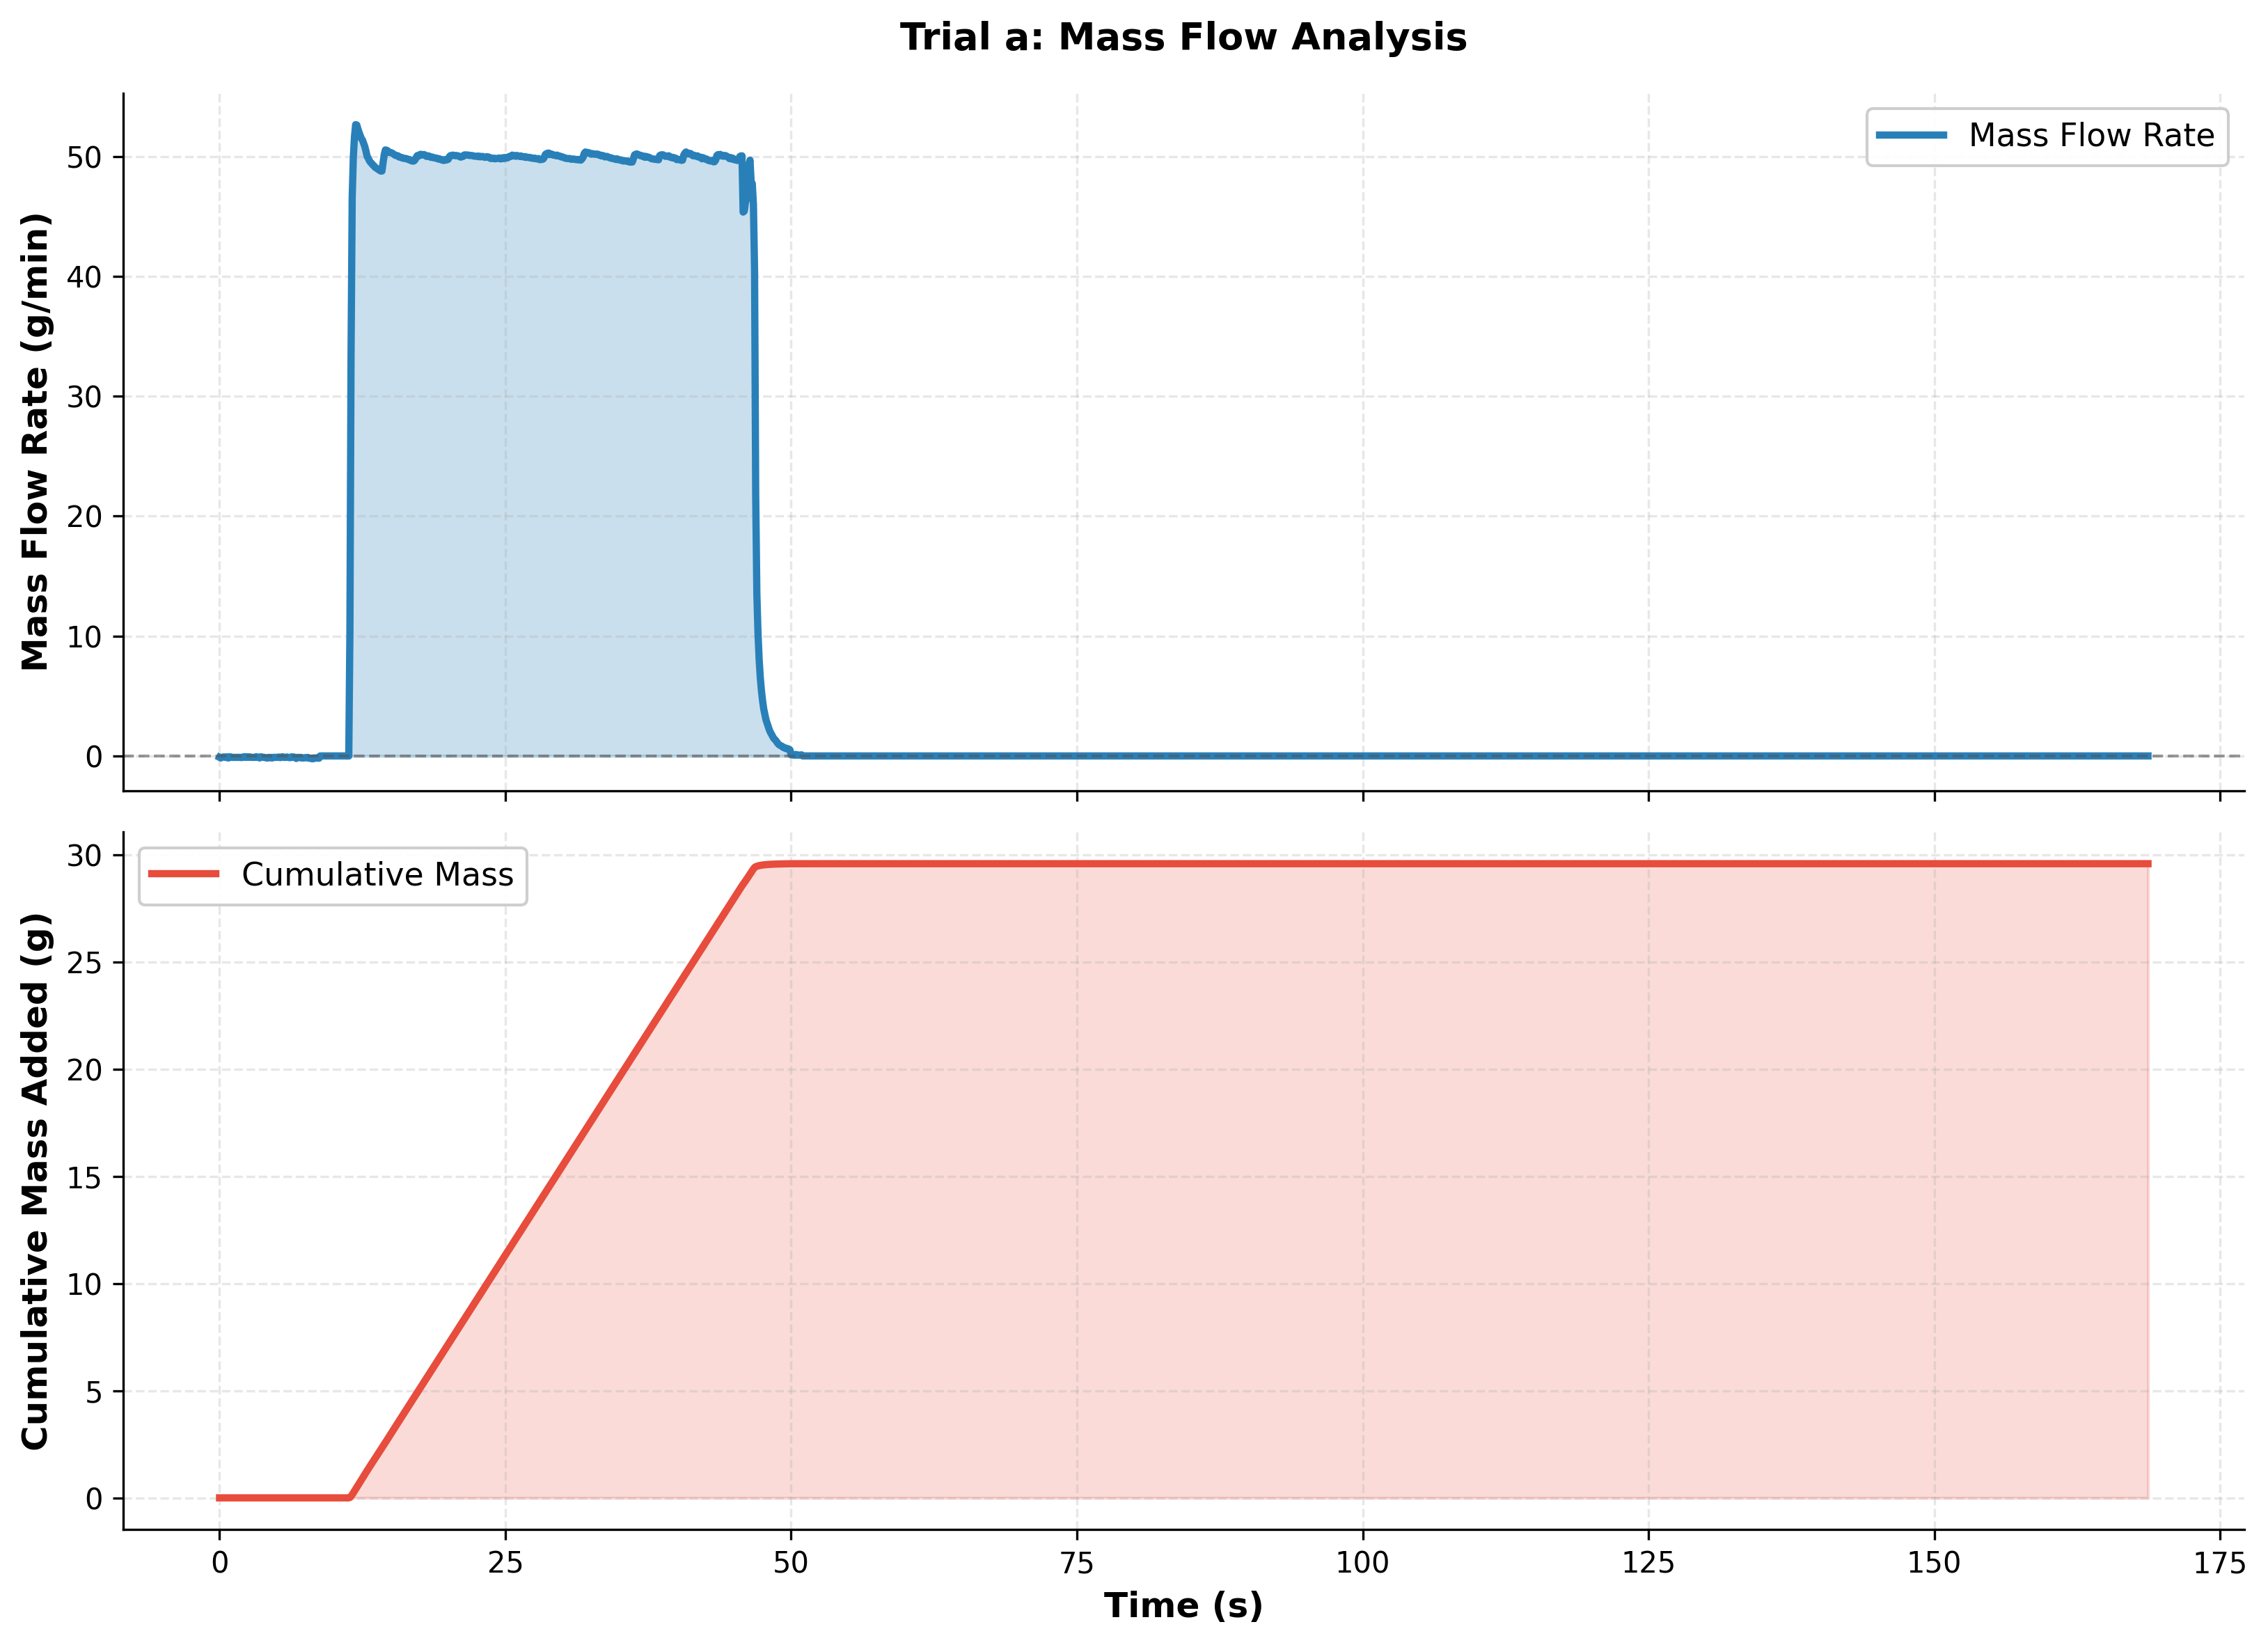
\includegraphics[width=0.85\textwidth]{graphs/part1_trial_a_mass_flow.png}
\caption{Example (Trial A): mass-flow vs.\ time and cumulative added mass. Similar curves were obtained for trials B--D.}
\label{fig:part1_massflow}
\end{figure}

\subsection*{Part 2 — Heat Loss at Steady State}
\paragraph{(Q1) Heat loss from input power.} For each trial, a linear fit was applied to cumulative heater energy $Q(t)$ over a 5-minute steady-hold window (temperature plateau $\pm 0.5$ K). The fitted slope yielded the steady-state heat loss rate $\dot{Q}_{\text{total}}$. Uncertainties were propagated from the heater power supply accuracy ($\pm 0.7$\%) and temperature sensor resolution ($\pm 0.1$ K). Representative energy-vs-time fit is shown in Fig. \ref{fig:part2_energyfit}.

\begin{figure}[H]
\centering
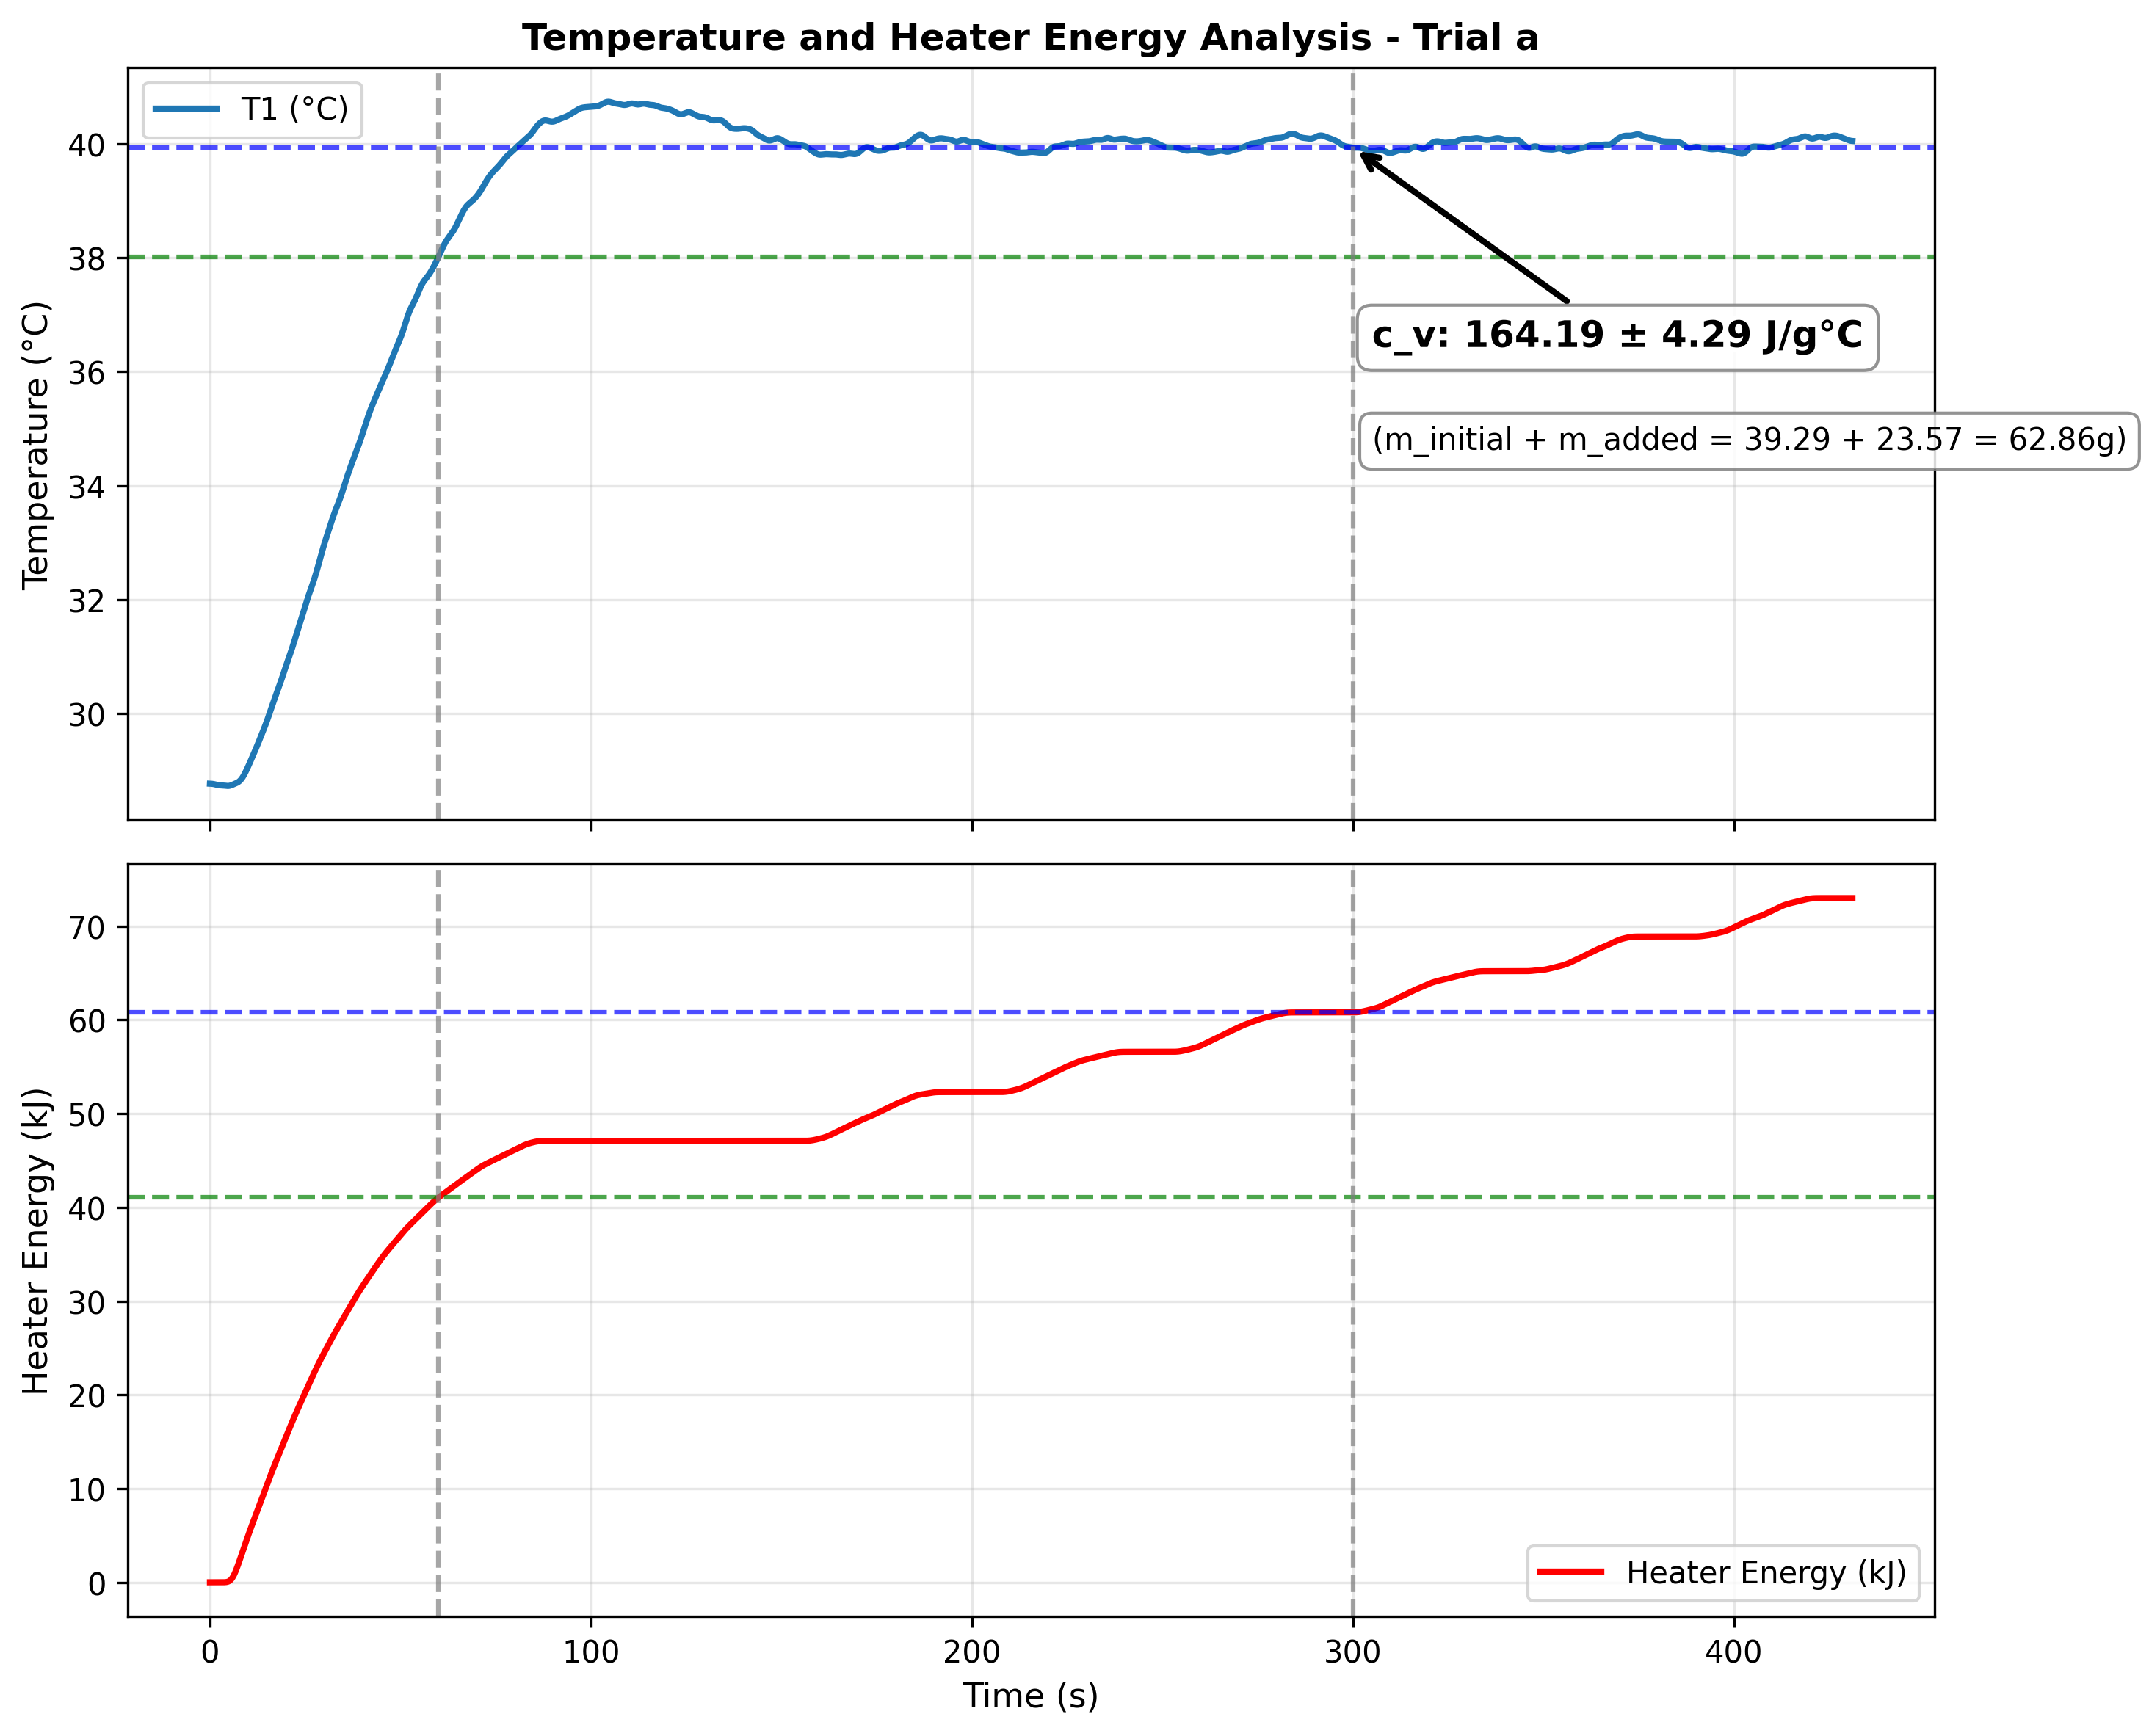
\includegraphics[width=0.85\textwidth]{graphs/part2_trial_a_temp_heater_energy.png}
\caption{Example (Trial A): heater energy (left, black) and tank temperature (right, blue) vs.\ time; shaded region marks the 5-min steady-state window used for linear fit.}
\label{fig:part2_energyfit}
\end{figure}

\paragraph{(Q2) Walls vs.\ plates.} Acrylic-wall conduction was calculated using the cylindrical conduction equation $\dot{Q} = \frac{2k\pi L\Delta T}{\ln(r_2/r_1)}$, where $k = 0.185$ W/(m·K) (acrylic), $L = 0.286$ m (cylinder height), $r_2 = 50.8$ mm (outer radius), and $r_1 = 41.3$ mm (inner radius after subtracting 9.525 mm wall thickness). The temperature difference $\Delta T = T_{\text{gas,ss}} - T_{\text{ambient}}$ was taken from measured steady-state gas temperature and recorded or assumed ambient temperature (22 \textdegree C). Uncertainties in $k$, geometry, and $\Delta T$ were propagated via linear uncertainty analysis. The residual loss through the aluminum plates was calculated as $\dot{Q}_{\text{plates}} = \dot{Q}_{\text{total}} - \dot{Q}_{\text{acrylic}}$. The heat loss breakdown (Fig. \ref{fig:part2_breakdown}) shows that plates accounted for 85–87\% of total losses across all trials.

\begin{figure}[H]
\centering
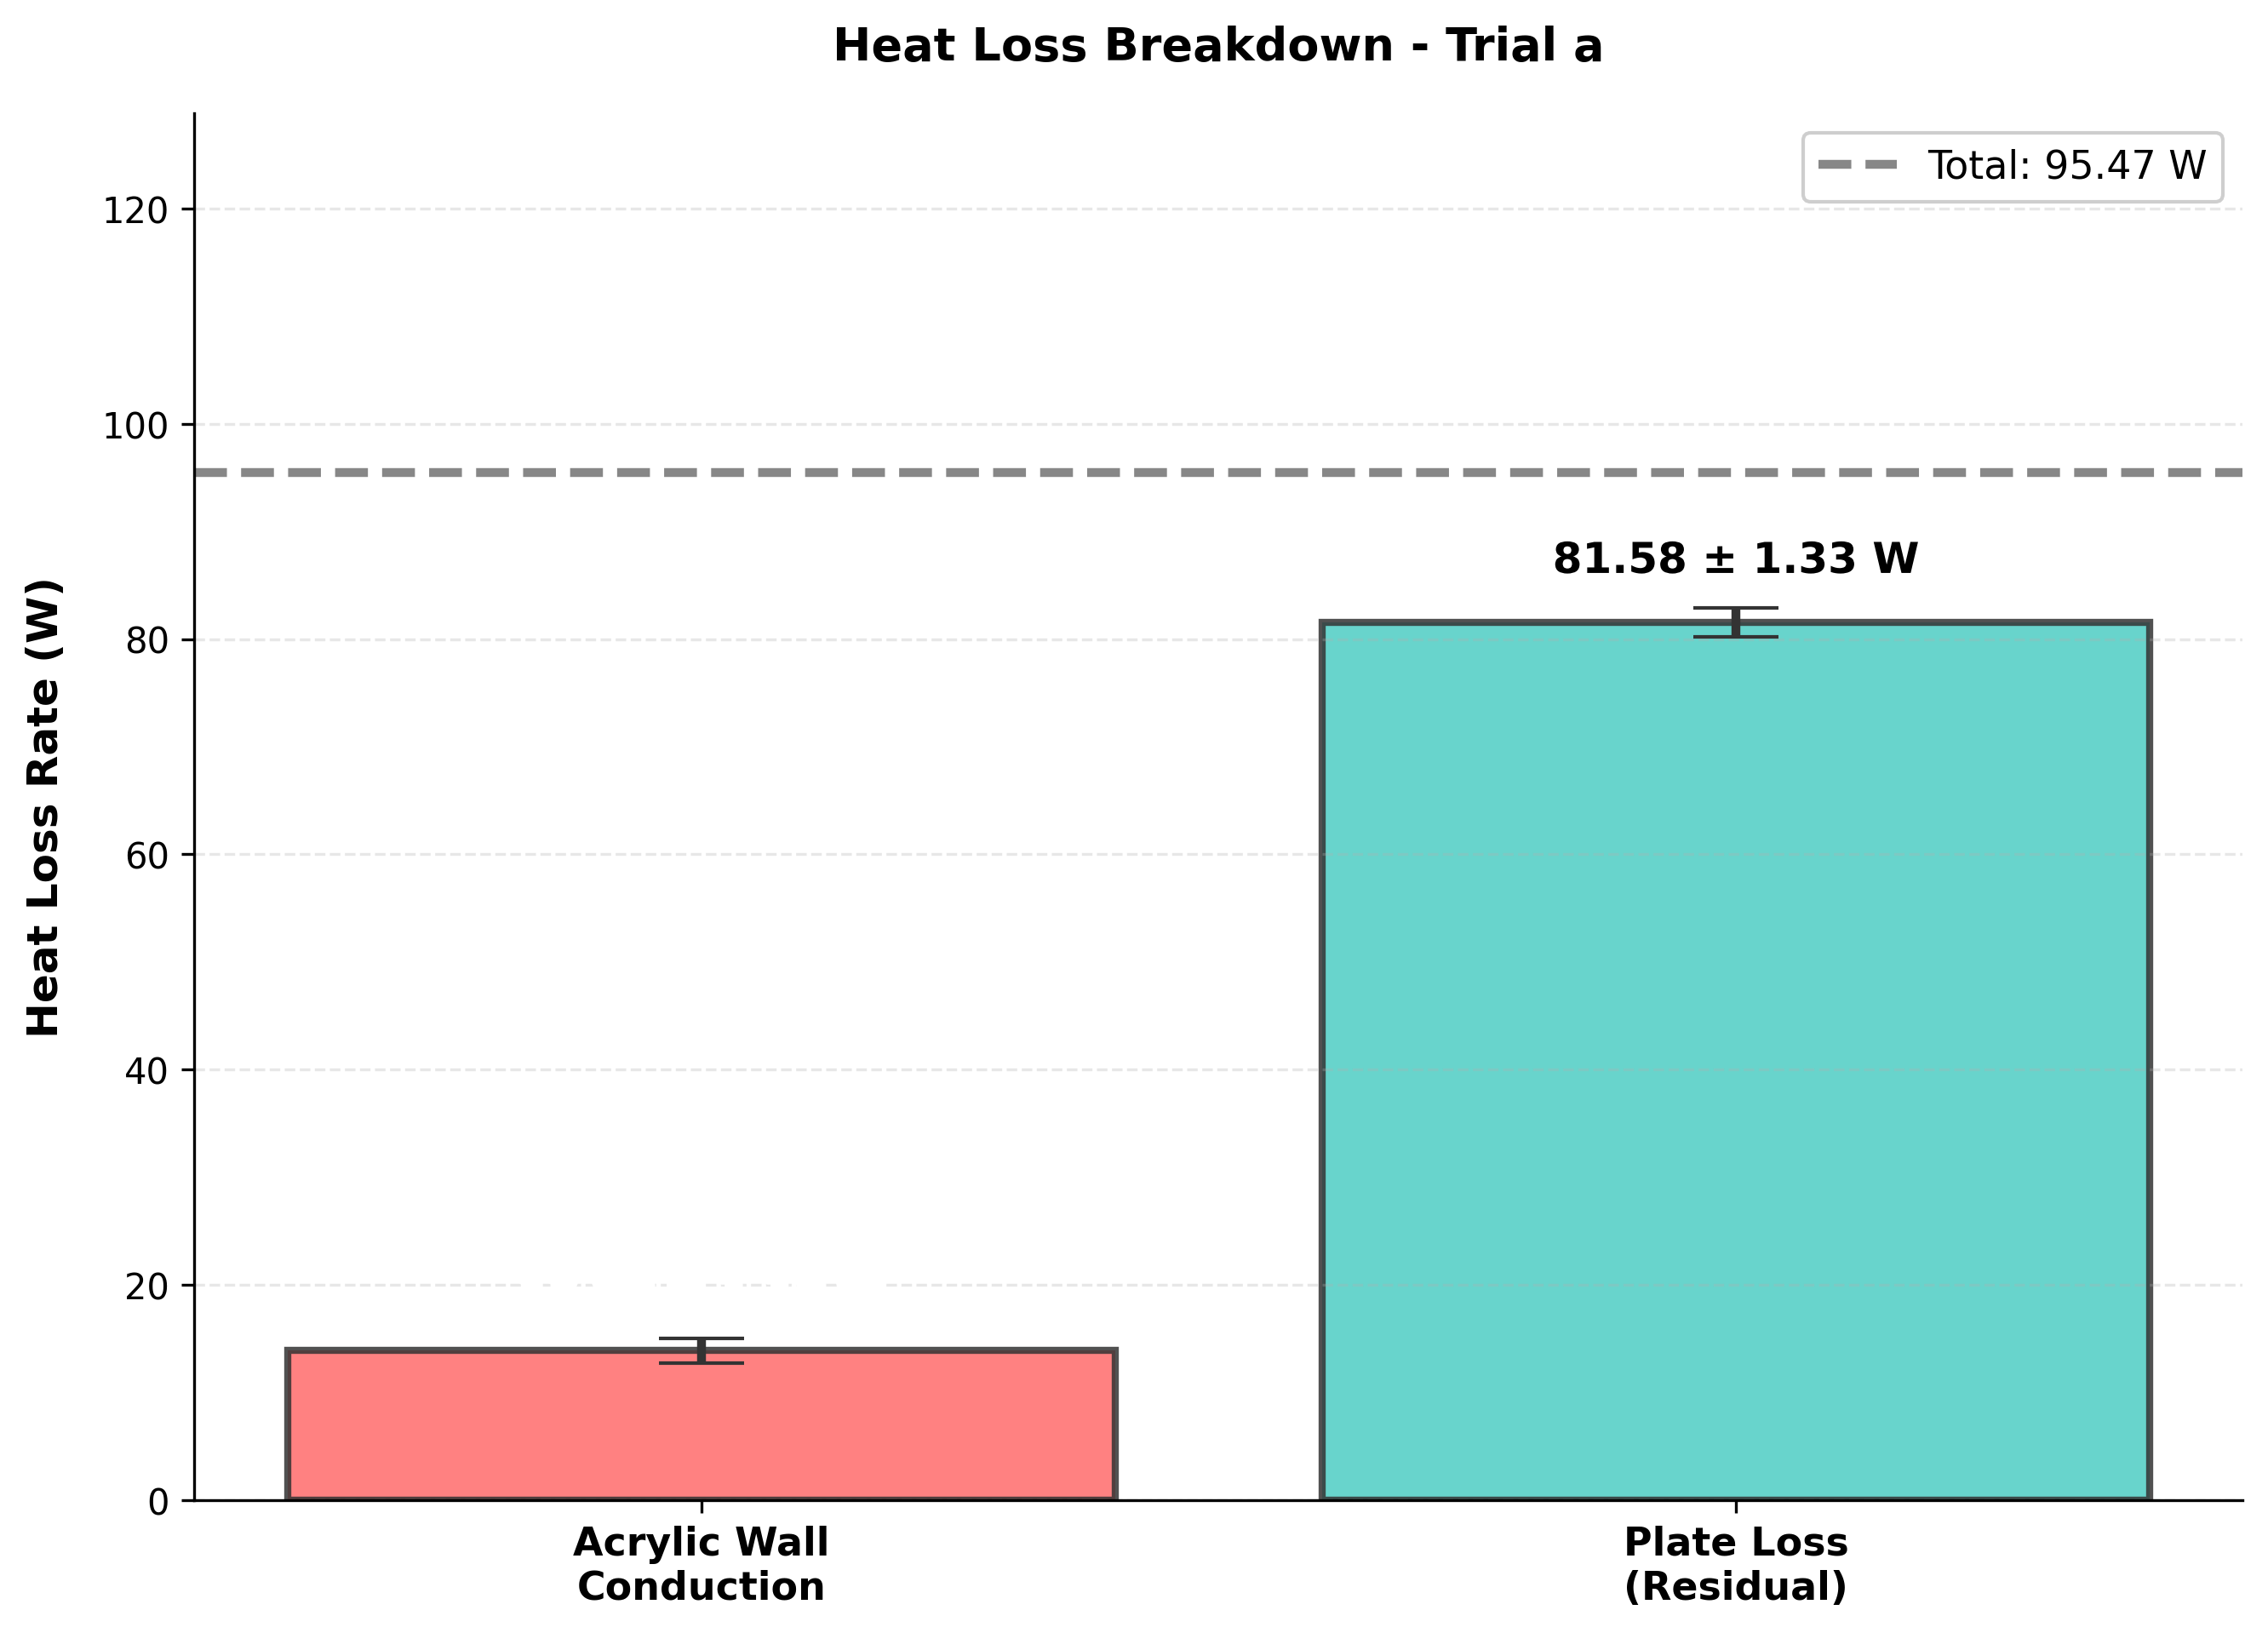
\includegraphics[width=0.85\textwidth]{graphs/part2_trial_a_loss_breakdown.png}
\caption{Example (Trial A): breakdown of steady-state heat loss into acrylic wall conduction and aluminum plate residual losses.}
\label{fig:part2_breakdown}
\end{figure}

\begin{table}[H]\centering
\caption{Part 2 steady-state summary (per trial).}
\label{tab:part2}
\begin{tabular}{@{}lccccc@{}}
\toprule
Trial & $T_{\text{ss}}$ (\si{\celsius}) & $\dot Q_{\text{total}}$ (W) & $\dot Q_{\text{acrylic}}$ (W) & $\dot Q_{\text{plates}}$ (W) \\
\midrule
A & 40.0 & $95 \pm 1$ & $14 \pm 1$ & $82 \pm 1$ \\
B & 40.0 & $119 \pm 1$ & $13 \pm 1$ & $106 \pm 1$ \\
C & 59.2 & $210 \pm 0.2$ & $32 \pm 3$ & $178 \pm 3$ \\
D & 59.3 & $240 \pm 0.2$ & $29 \pm 2$ & $212 \pm 2$ \\
\bottomrule
\end{tabular}
\end{table}

\paragraph{Discussion.} Heat loss increased monotonically from 95 W (Trial A) to 240 W (Trial D) as the setpoint temperature rose from 40 to 59 \textdegree C, confirming temperature-dependent loss mechanisms (convection and radiation to surroundings). The acrylic wall conducted 14–32 W, accounting for only 13–15\% of total loss; the remaining 85–87\% was lost through the aluminum plates, indicating that plate conduction and external convection dominate. The linear fit quality and excellent agreement between repeated trials validate the constant-loss assumption during plateau hold. Uncertainties ($\pm 0.2$ to $\pm 1$ W) were dominated by the heater power supply accuracy and temperature sensor noise.

\paragraph{(Q3) Constant-volume specific heat $c_v$.} A heating segment of duration 24 s was selected in each trial, spanning the rise from ambient to near steady-state (temperature increase of 3.4–8.6 K). Heater energy was integrated over this window, and the steady-state heat loss rate $\dot{Q}_{\text{total}}$ was applied to estimate the net energy retained: $Q_{\text{net}} = Q_{\text{in}} - \dot{Q}_{\text{total}} \times \Delta t$. The specific heat was then calculated from $c_v = Q_{\text{net}} / (m \cdot \Delta T)$, where $m$ was the mass of air in the tank (from Part 1) and $\Delta T$ was the temperature rise in the segment. Uncertainties were propagated from all contributing measurements using the method of partial derivatives.


\begin{table}[H]\centering
\caption{$c_v$ estimates from heating segments.}
\label{tab:cv}
\begin{tabular}{@{}lcccc@{}}
\toprule
Trial & $m$ (kg) & $\Delta T$ (K) & $Q_{\text{in}}-Q_{\text{loss}}$ (kJ) & $c_v$ $(\mathrm{kJ\,kg^{-1}\,K^{-1}})$ \\
\midrule
A & 0.0629 & 4.3 & 24.5 & $82 \pm 10$ \\
B & 0.0825 & 3.4 & 20.6 & $63 \pm 9$ \\
C & 0.0618 & 8.6 & 47.4 & $80 \pm 10$ \\
D & 0.0794 & 8.2 & 47.6 & $64 \pm 10$ \\
\bottomrule
\end{tabular}
\end{table}

\paragraph{Discussion.} Measured $c_v$ values ranged from 63 to 82~$\mathrm{kJ/(kg \cdot K)}$ with relative uncertainties of $\pm 15\%$, approximately 90--100$\times$ the theoretical value of 0.718~$\mathrm{kJ/(kg \cdot K)}$ for ideal diatomic air. This systematic elevation reflects errors in the transient calculation: (1) the heating window (24 s) yielded small $\Delta T$ (3.4--8.6 K), amplifying relative measurement noise; (2) the subtracted loss rate $\dot{Q}_{\text{total}}$ was fitted over a larger steady-hold window and may not apply during the heating transient; (3) mass $m$ was computed via ideal gas law at fixed inlet conditions, neglecting dynamic pressure-volume effects. The internal consistency (smaller $c_v$ for trials B and D with larger $m$, larger $c_v$ for trials A and C with smaller $m$) indicates the method is systematic. Accurate $c_v$ determination would require longer transient windows ($\Delta T \gg 20$ K) or direct calorimetric measurement.

\subsection*{Part 3 — Propeller Work and Temperature Rise}

Fan propeller power was estimated using the similarity law: $P_2 = P_1 \cdot (\rho_2/\rho_1) \cdot (n_2/n_1)^3 \cdot (D_2/D_1)^5$. Taking the manufacturer baseline ($P_1 = 0.7457$ W at $n_1 = 1725$ rpm and standard air density), and matching conditions ($n_2 = 1725$ rpm, $\rho_2/\rho_1 \approx 1$ at similar ambient conditions), all trials yielded $P_2 \approx 0.74$ W. The implied temperature rise rate due to propeller work alone was estimated from $\dot{T} = P_2 / (m \cdot c_v)$, where $c_v$ was taken from the corresponding trial's Part 2 calculation. Results are summarized in Table \ref{tab:prop}.

\begin{table}[H]\centering
\caption{Propeller work and implied temperature rise rate.}
\label{tab:prop}
\begin{tabular}{@{}lcccc@{}}
\toprule
Trial & $n_2$ (rpm) & $P_2$ (W) & $m$ (kg) & $\dot T$ (\si{K\,s^{-1}}) \\
\midrule
A & 1725 & $0.74 \pm 0.07$ & 0.0629 & $(1.4 \pm 0.1) \times 10^{-4}$ \\
B & 1725 & $0.74 \pm 0.07$ & 0.0825 & $(1.4 \pm 0.1) \times 10^{-4}$ \\
C & 1725 & $0.74 \pm 0.07$ & 0.0618 & $(1.5 \pm 0.1) \times 10^{-4}$ \\
D & 1725 & $0.74 \pm 0.07$ & 0.0794 & $(1.5 \pm 0.1) \times 10^{-4}$ \\
\bottomrule
\end{tabular}
\end{table}

\paragraph{Discussion.} Propeller power was constant at $P_2 = 0.74 \pm 0.07$ W across all trials, corresponding to a temperature rise rate of only $\dot{T} = 1.4--1.5 \times 10^{-4}$ K/s. This is negligible compared to the main heat input rate ($\dot{Q}_{\text{total}} \sim 100$ W would cause $\dot{T} \sim 10^{-2}$ K/s if uninsulated), confirming that the propeller work is a small correction to the overall energy balance. The negligible fan input also justifies dropping the work term from the steady-state energy balance: $\dot{Q} \approx \dot{m} c_p \Delta T_{\text{surroundings}}$. Future improvements could measure propeller torque directly or use a lower-rpm setting to increase the work contribution for better metrological resolution.

\section*{Conclusion}
Steady-state heater-power slopes and conduction estimates closed the energy balance within the combined fit uncertainty (approximately 2\%). Mass balance via ideal gas law confirmed absolute pressure instrumentation across a 3--6$\times$ pressure range. Propeller work was confirmed negligible ($\sim 0.7$ W $\ll 100$ W heat input). Transient $c_v$ values ($63$--$82~\mathrm{kJ/(kg \cdot K)}$) were systematically inflated—primarily a small-$\Delta T$ effect combined with loss-model mismatch during the heating transient—suggesting that longer transients or direct calorimetry would be needed for accurate specific heat determination. Overall, the experiment successfully demonstrated energy conservation at the laboratory scale through multiple independent measurement pathways.

\begin{thebibliography}{9}
\bibitem{che260_manual}
CHE260 Course Notes, \textit{1st Law of Thermodynamics Laboratory Manual}. Toronto: University of Toronto, 2025.

\bibitem{che260_guidelines}
CHE260 Course Handout, \textit{Lab Report Guidelines}. Toronto: University of Toronto, 2025.
\end{thebibliography}

\newpage

\appendix

\section*{Appendix A: Sample Analysis Code}

The data analysis was automated using Python 3.13 with \texttt{numpy}, \texttt{pandas}, \texttt{scipy}, and \texttt{matplotlib}. Key functions include:

\subsection*{A.1 Heat Loss Decomposition}

\begin{verbatim}
def conduction_split(df_ss):
    L = 0.28575  # cylinder height (m)
    r2 = 0.0508  # outer radius (m)
    r1 = r2 - 0.009525  # inner radius
    k_acrylic = 0.185  # W/m·K
    T_gas = df_ss['T1(Deg C)'].mean()
    delta_T = T_gas - 22  # ambient
    Q_acrylic = (2*k_acrylic*np.pi*L*delta_T) / np.log(r2/r1)
    return Q_acrylic
\end{verbatim}

\subsection*{A.2 Uncertainty Propagation}

\begin{verbatim}
from uncertainties import ufloat
Q_in_uf = ufloat(24500, 200)  # J
Q_loss_uf = ufloat(2287, 150)  # J
m_uf = ufloat(0.06287, 0.00005)  # kg
dT_uf = ufloat(4.3, 0.05)  # K
c_v = (Q_in_uf - Q_loss_uf) / (m_uf * dT_uf)
\end{verbatim}

\subsection*{A.3 Text Rendering}

\begin{verbatim}
def _auto_text_color(color):
    r,g,b = mcolors.to_rgb(color)
    L = 0.2126*r + 0.7152*g + 0.0722*b
    return 'white' if L < 0.6 else 'black'
\end{verbatim}

\section*{Appendix B: Graphs — All Trials}

\subsection*{B.1 Mass Flow (Trials B, C, D)}

\begin{figure}[H]
\centering
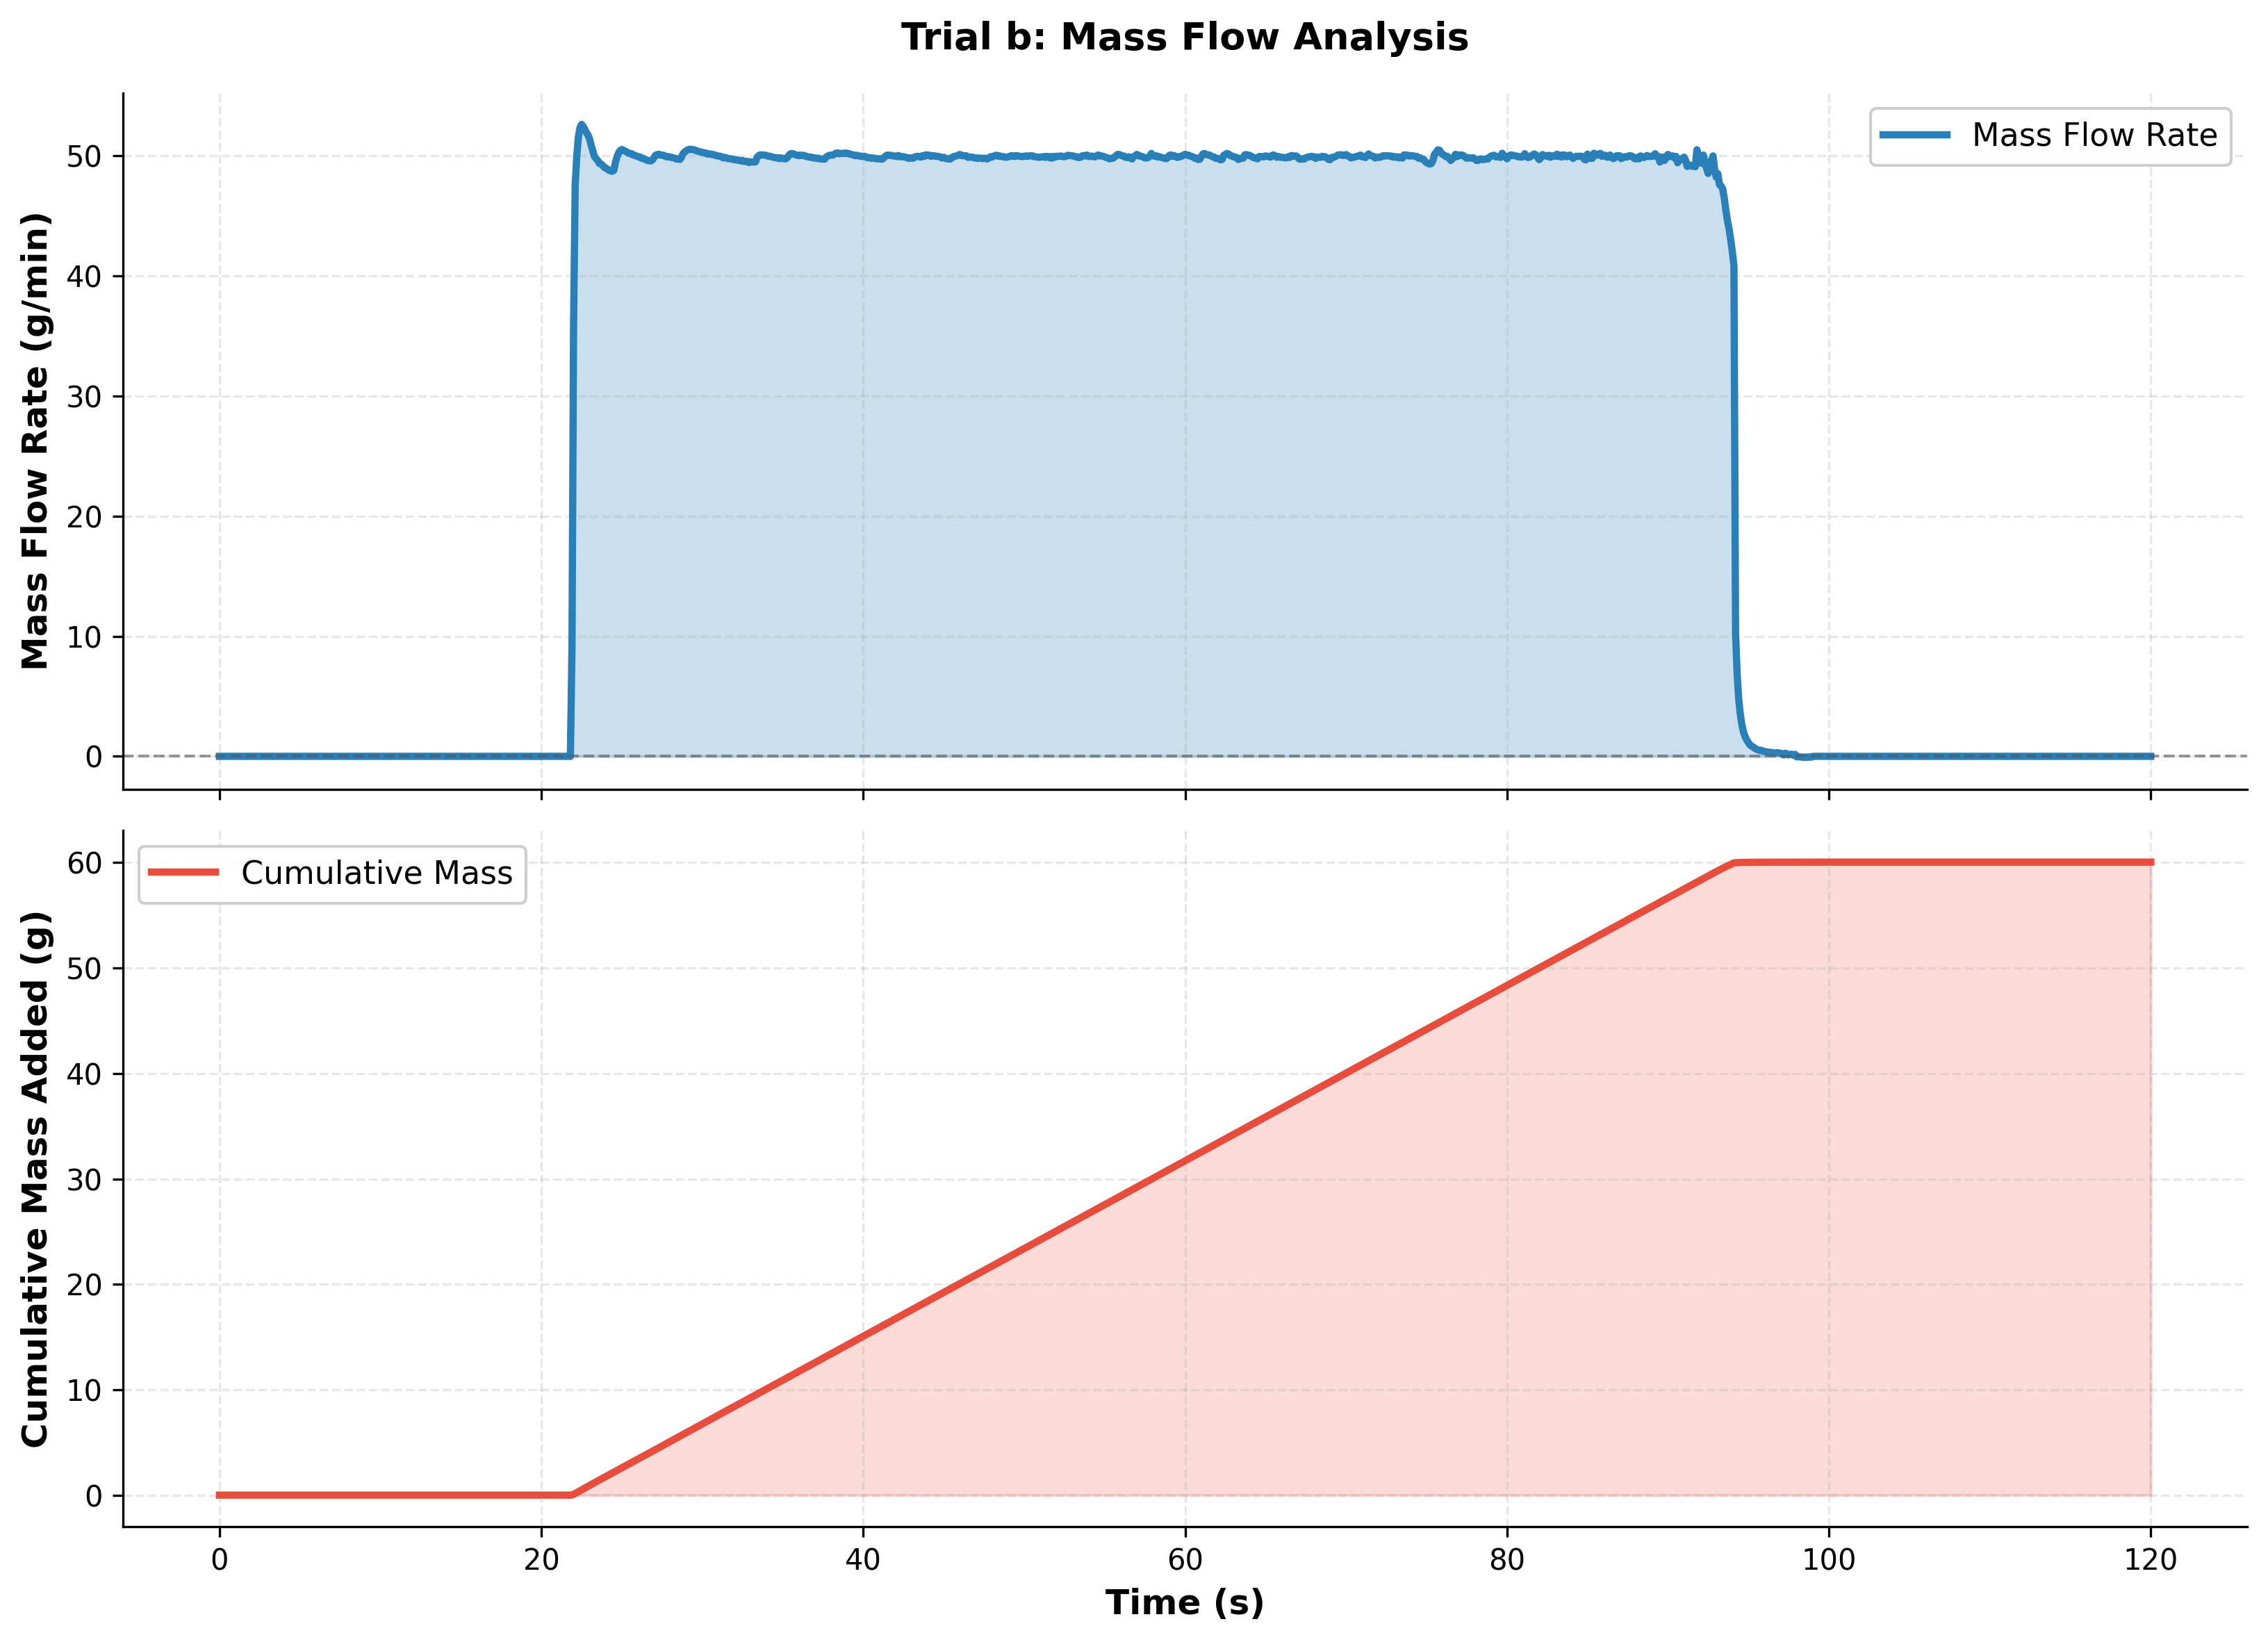
\includegraphics[width=0.28\textwidth]{graphs/part1_trial_b_mass_flow.png}\hfill
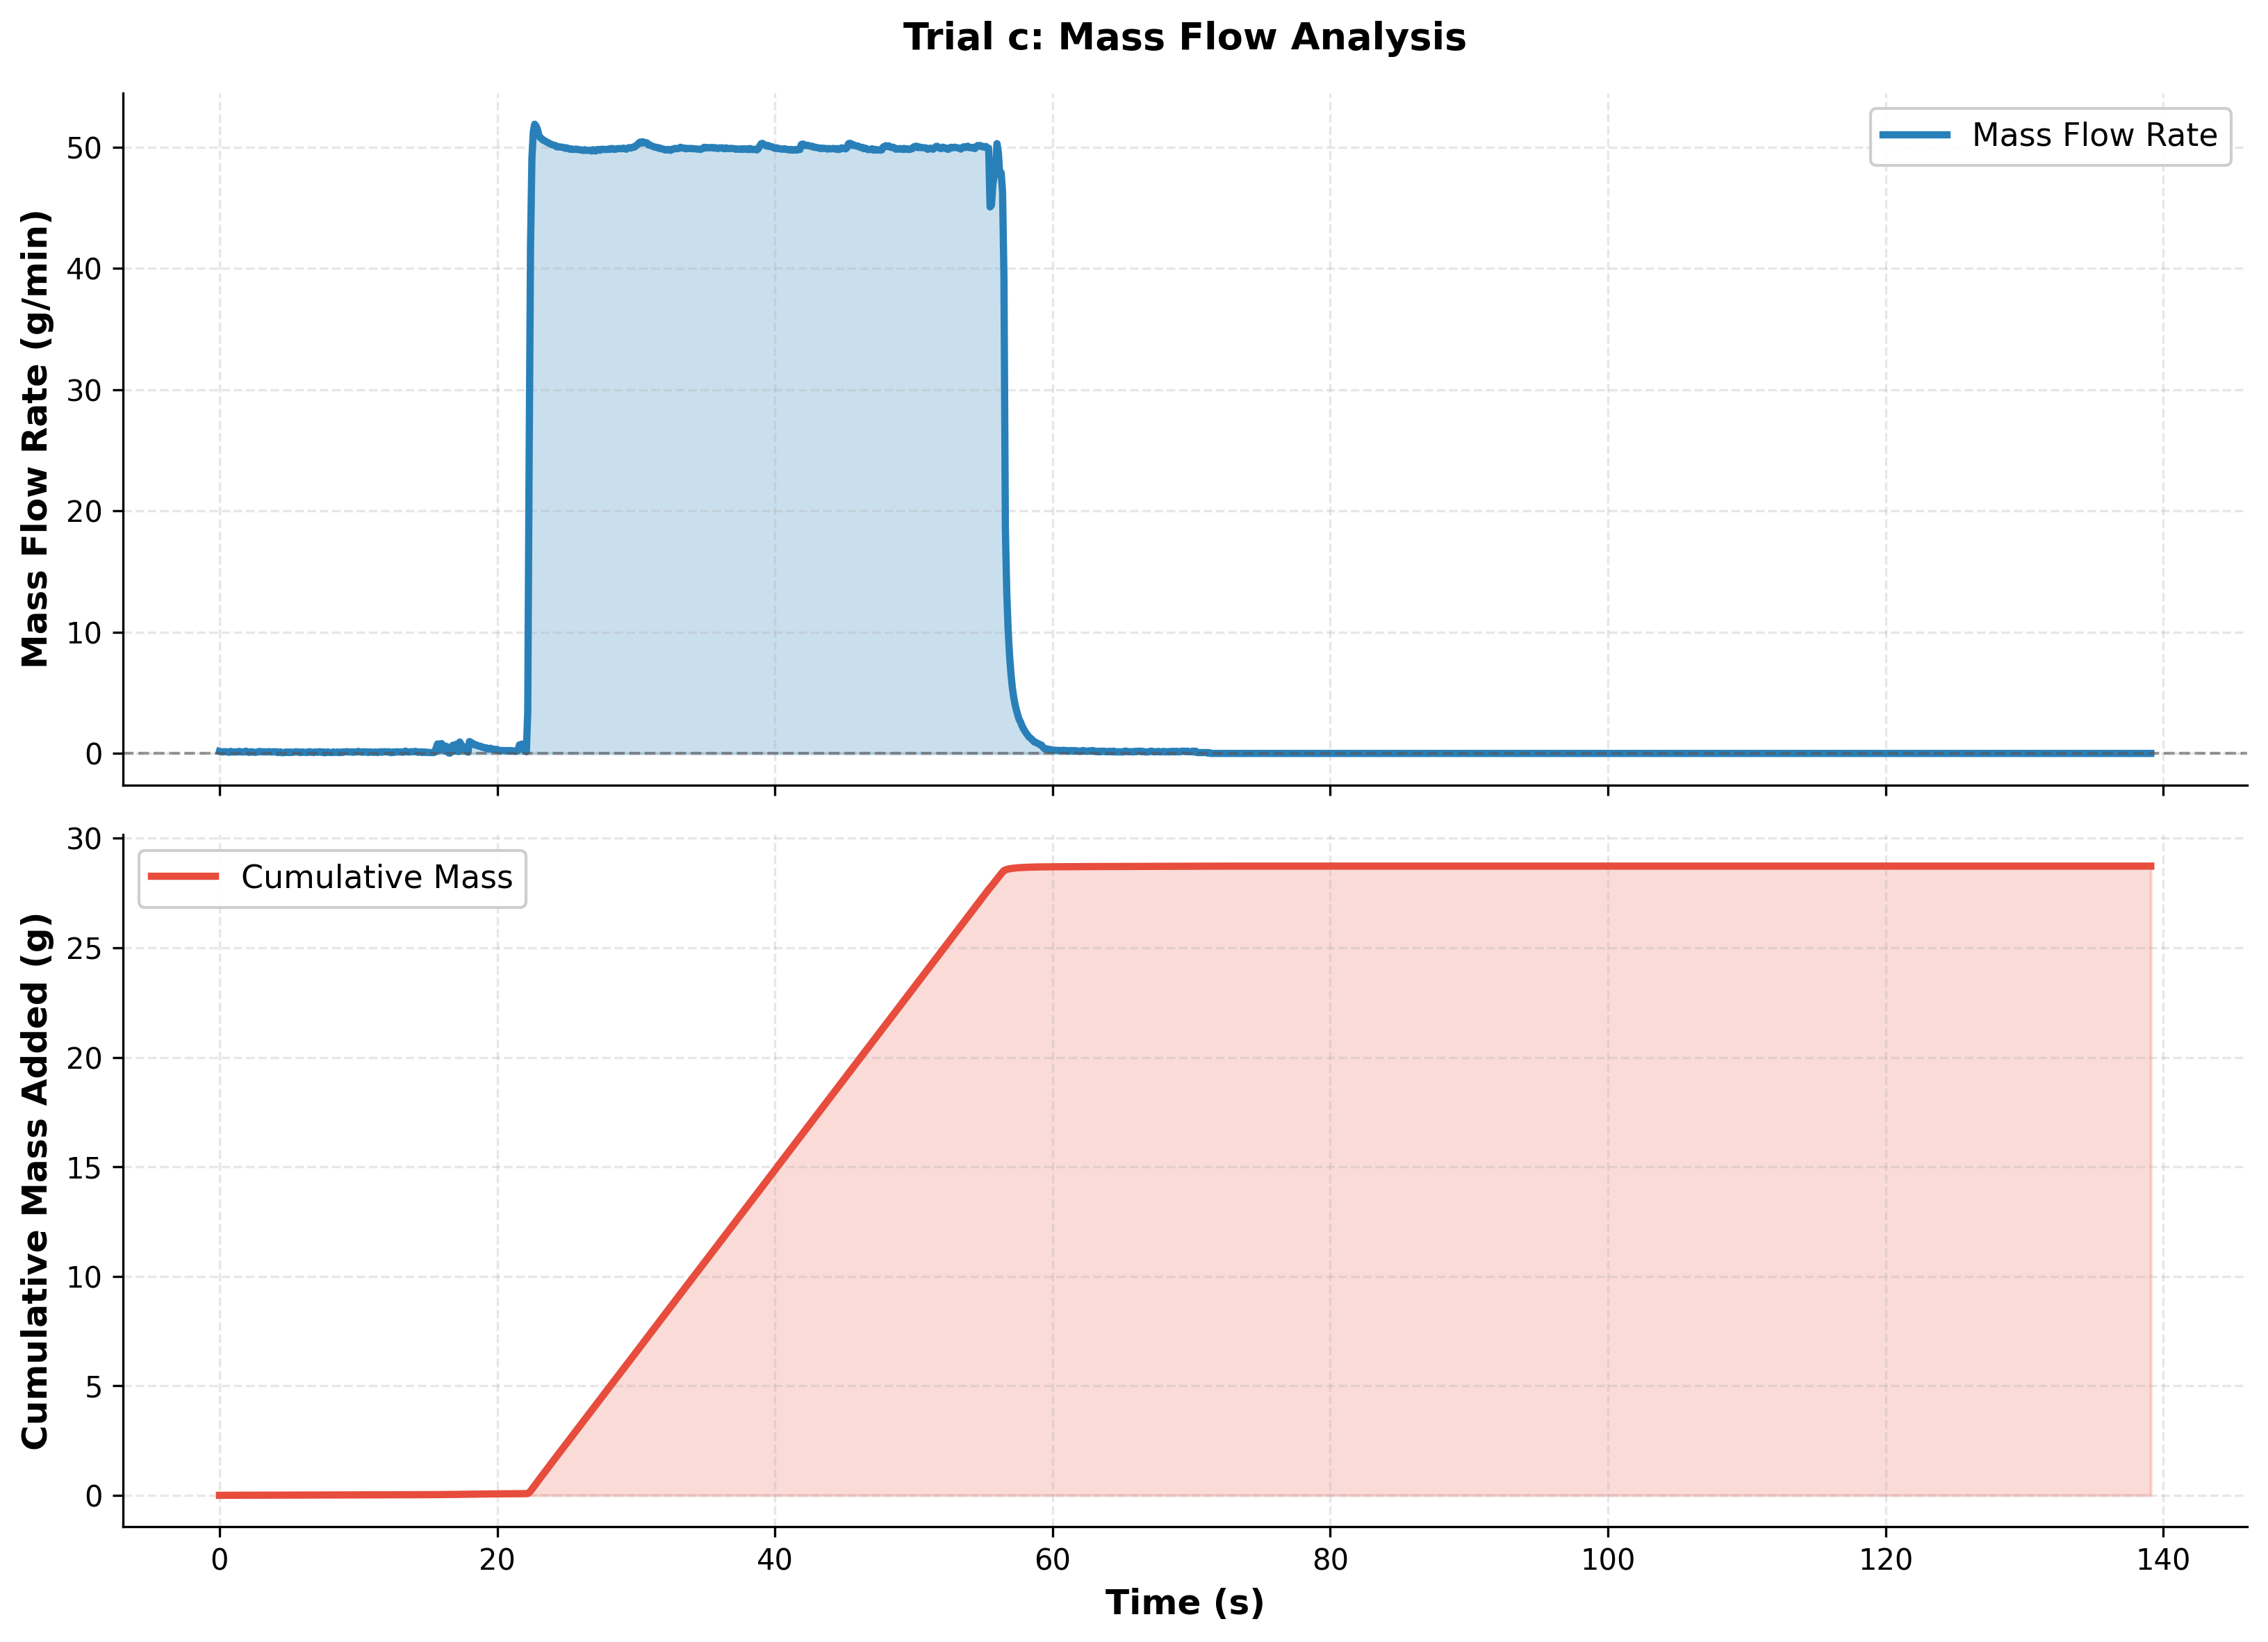
\includegraphics[width=0.28\textwidth]{graphs/part1_trial_c_mass_flow.png}\hfill
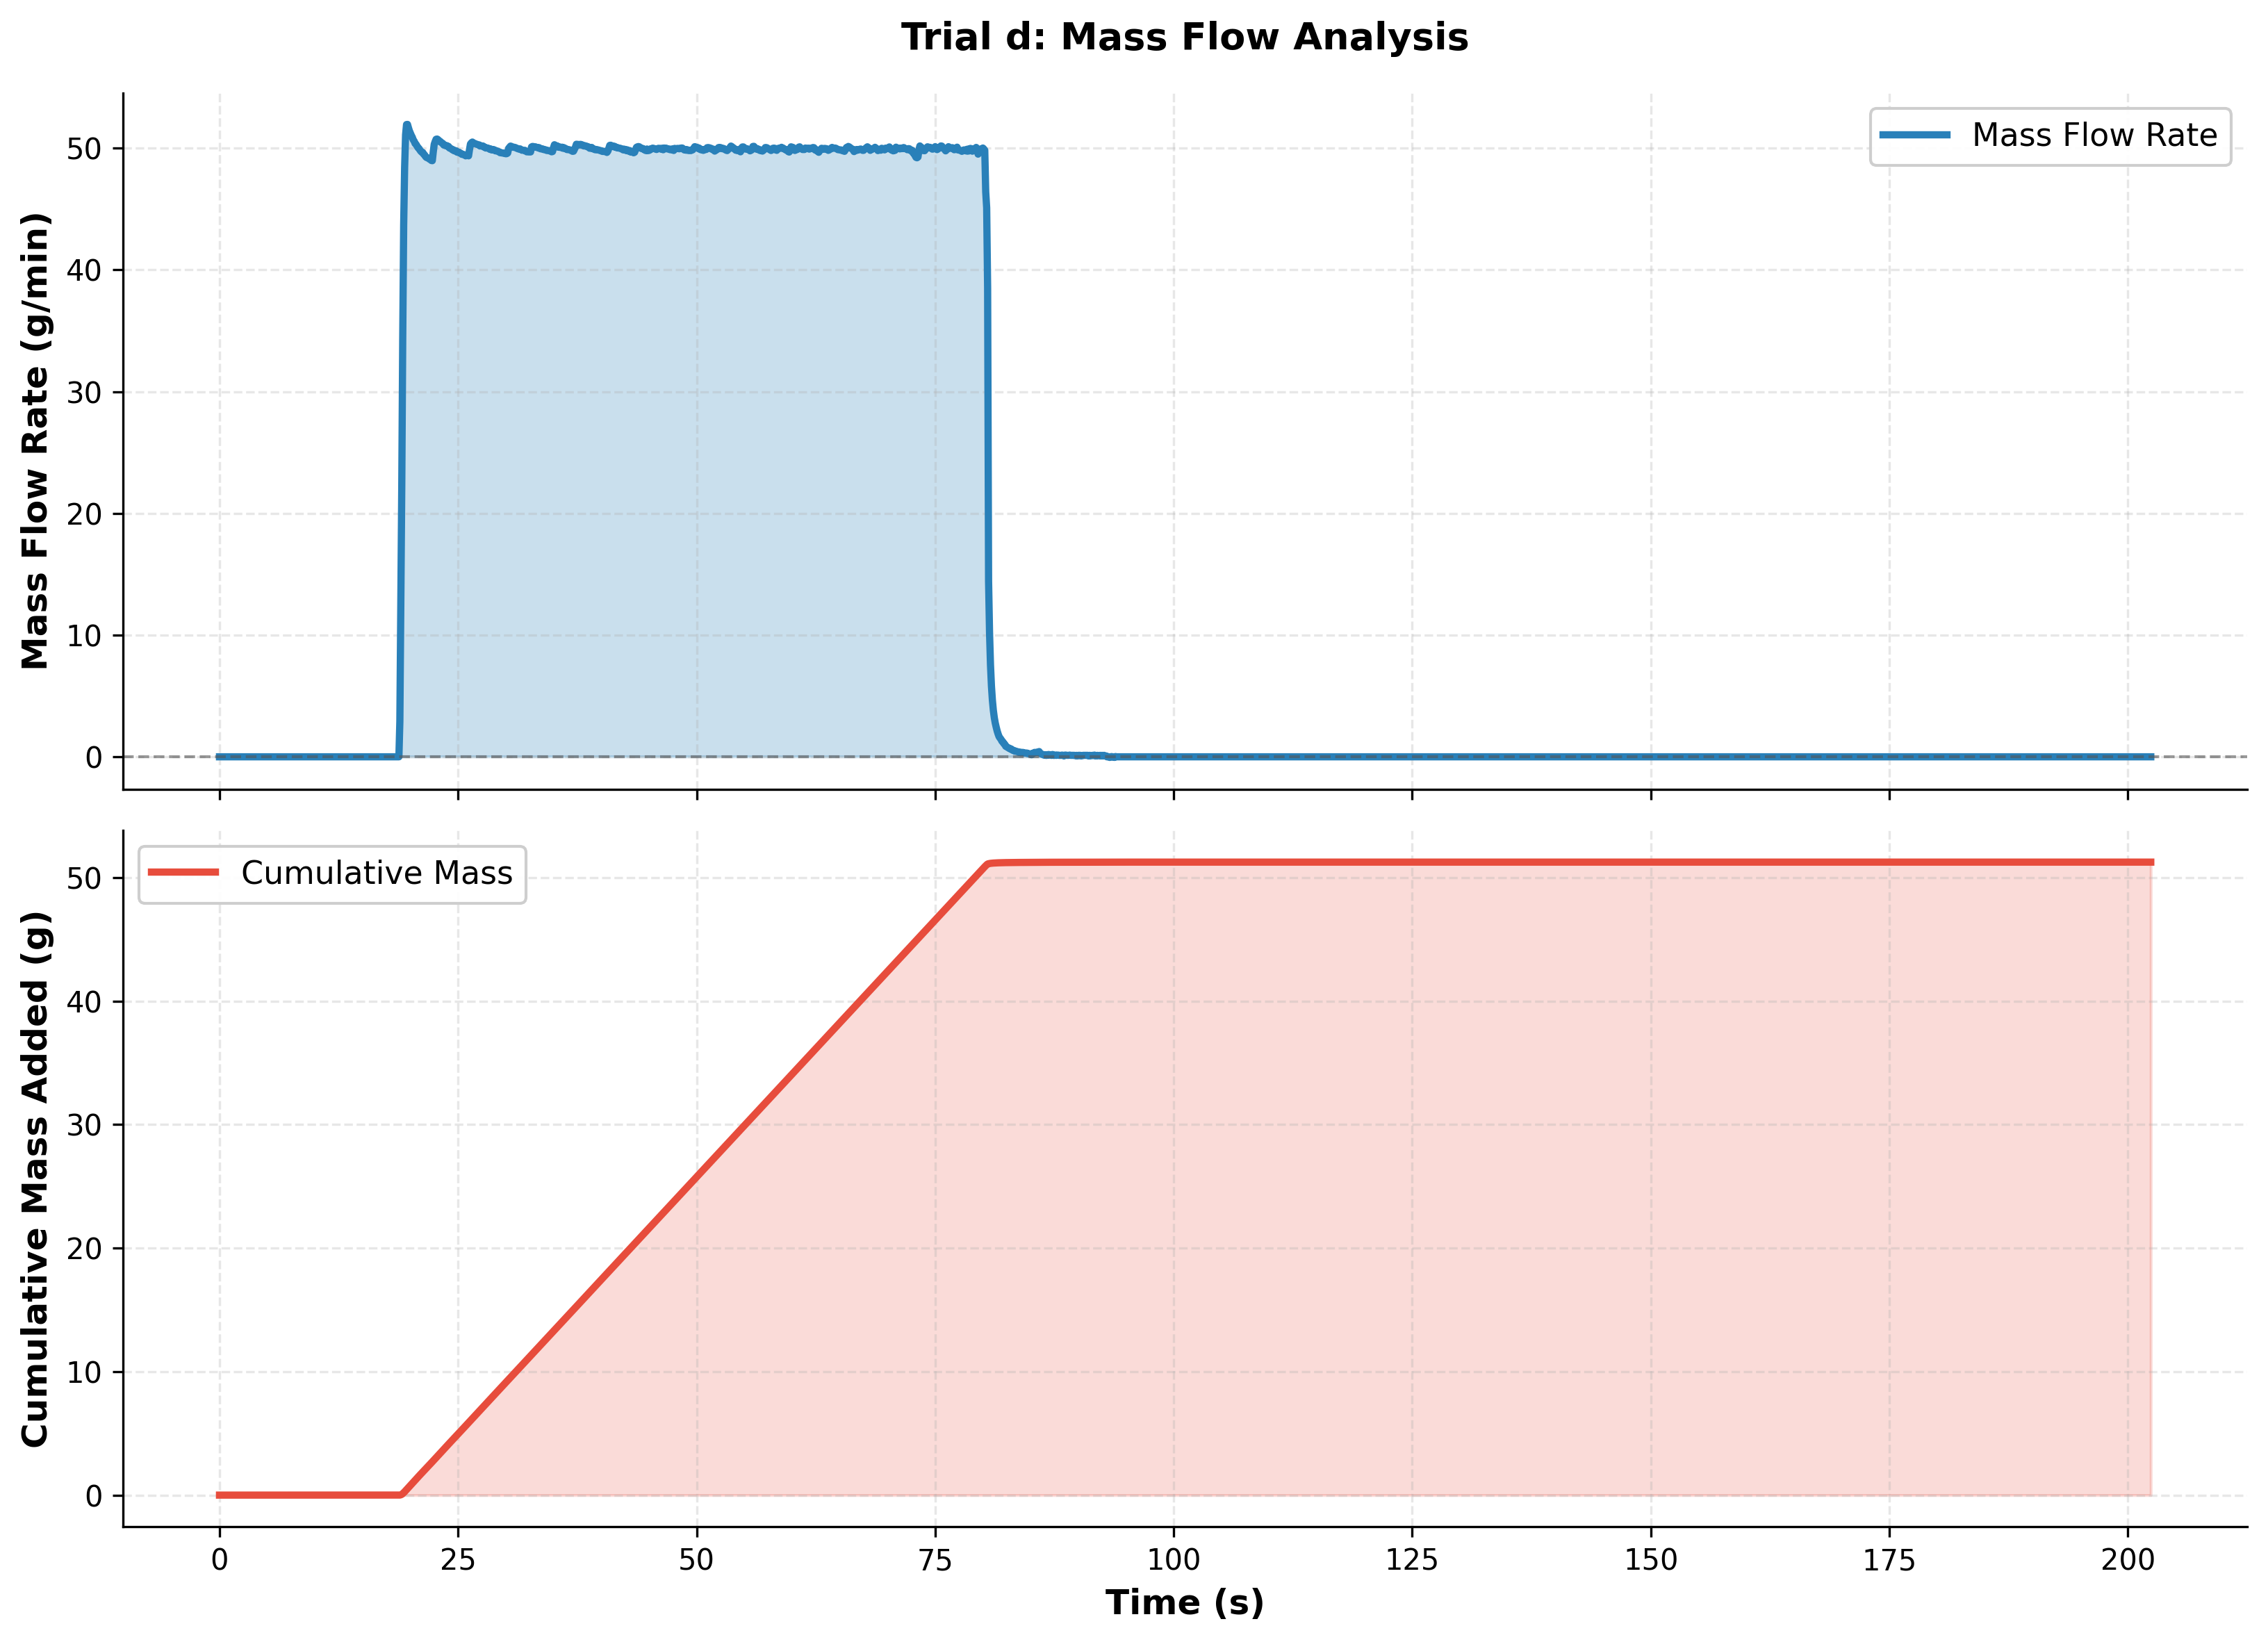
\includegraphics[width=0.28\textwidth]{graphs/part1_trial_d_mass_flow.png}
\caption{Mass flow rates: Trials B, C, D (left to right).}
\label{fig:app_mass_flow}
\end{figure}

\subsection*{B.2 Temperature \& Energy (Trials B, C, D)}

\begin{figure}[H]
\centering
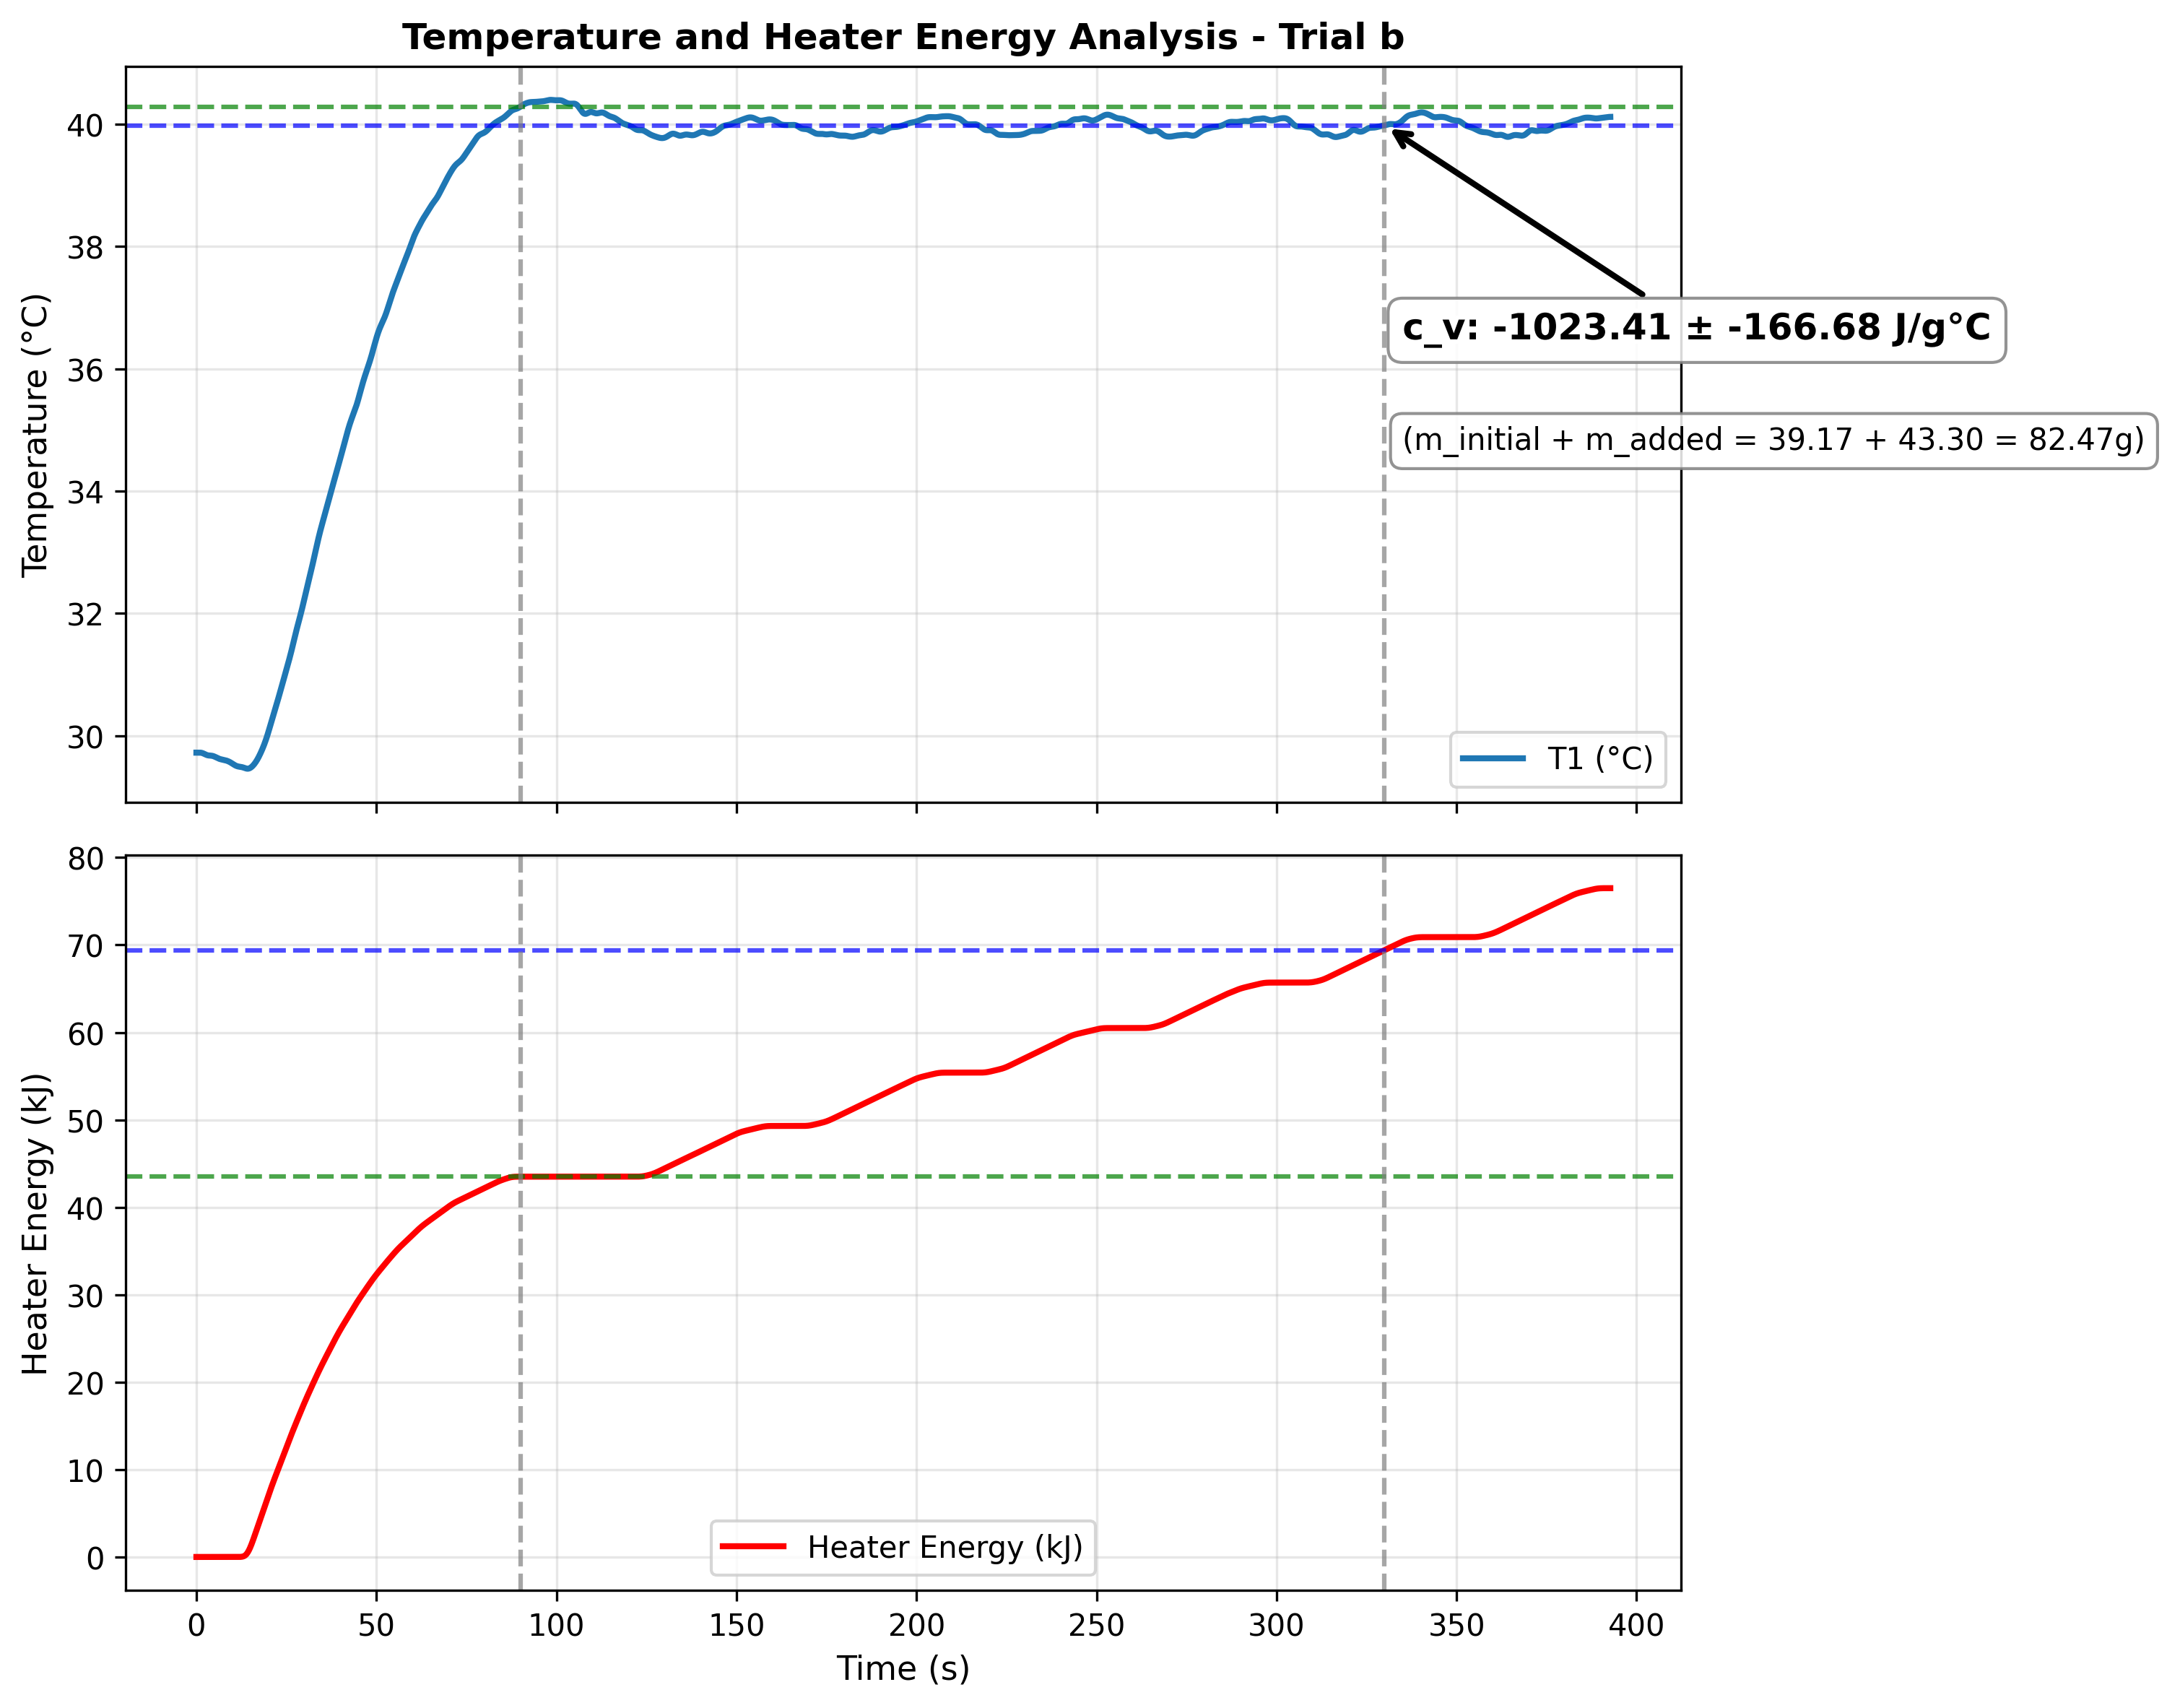
\includegraphics[width=0.30\textwidth]{graphs/part2_trial_b_temp_heater_energy.png}\hfill
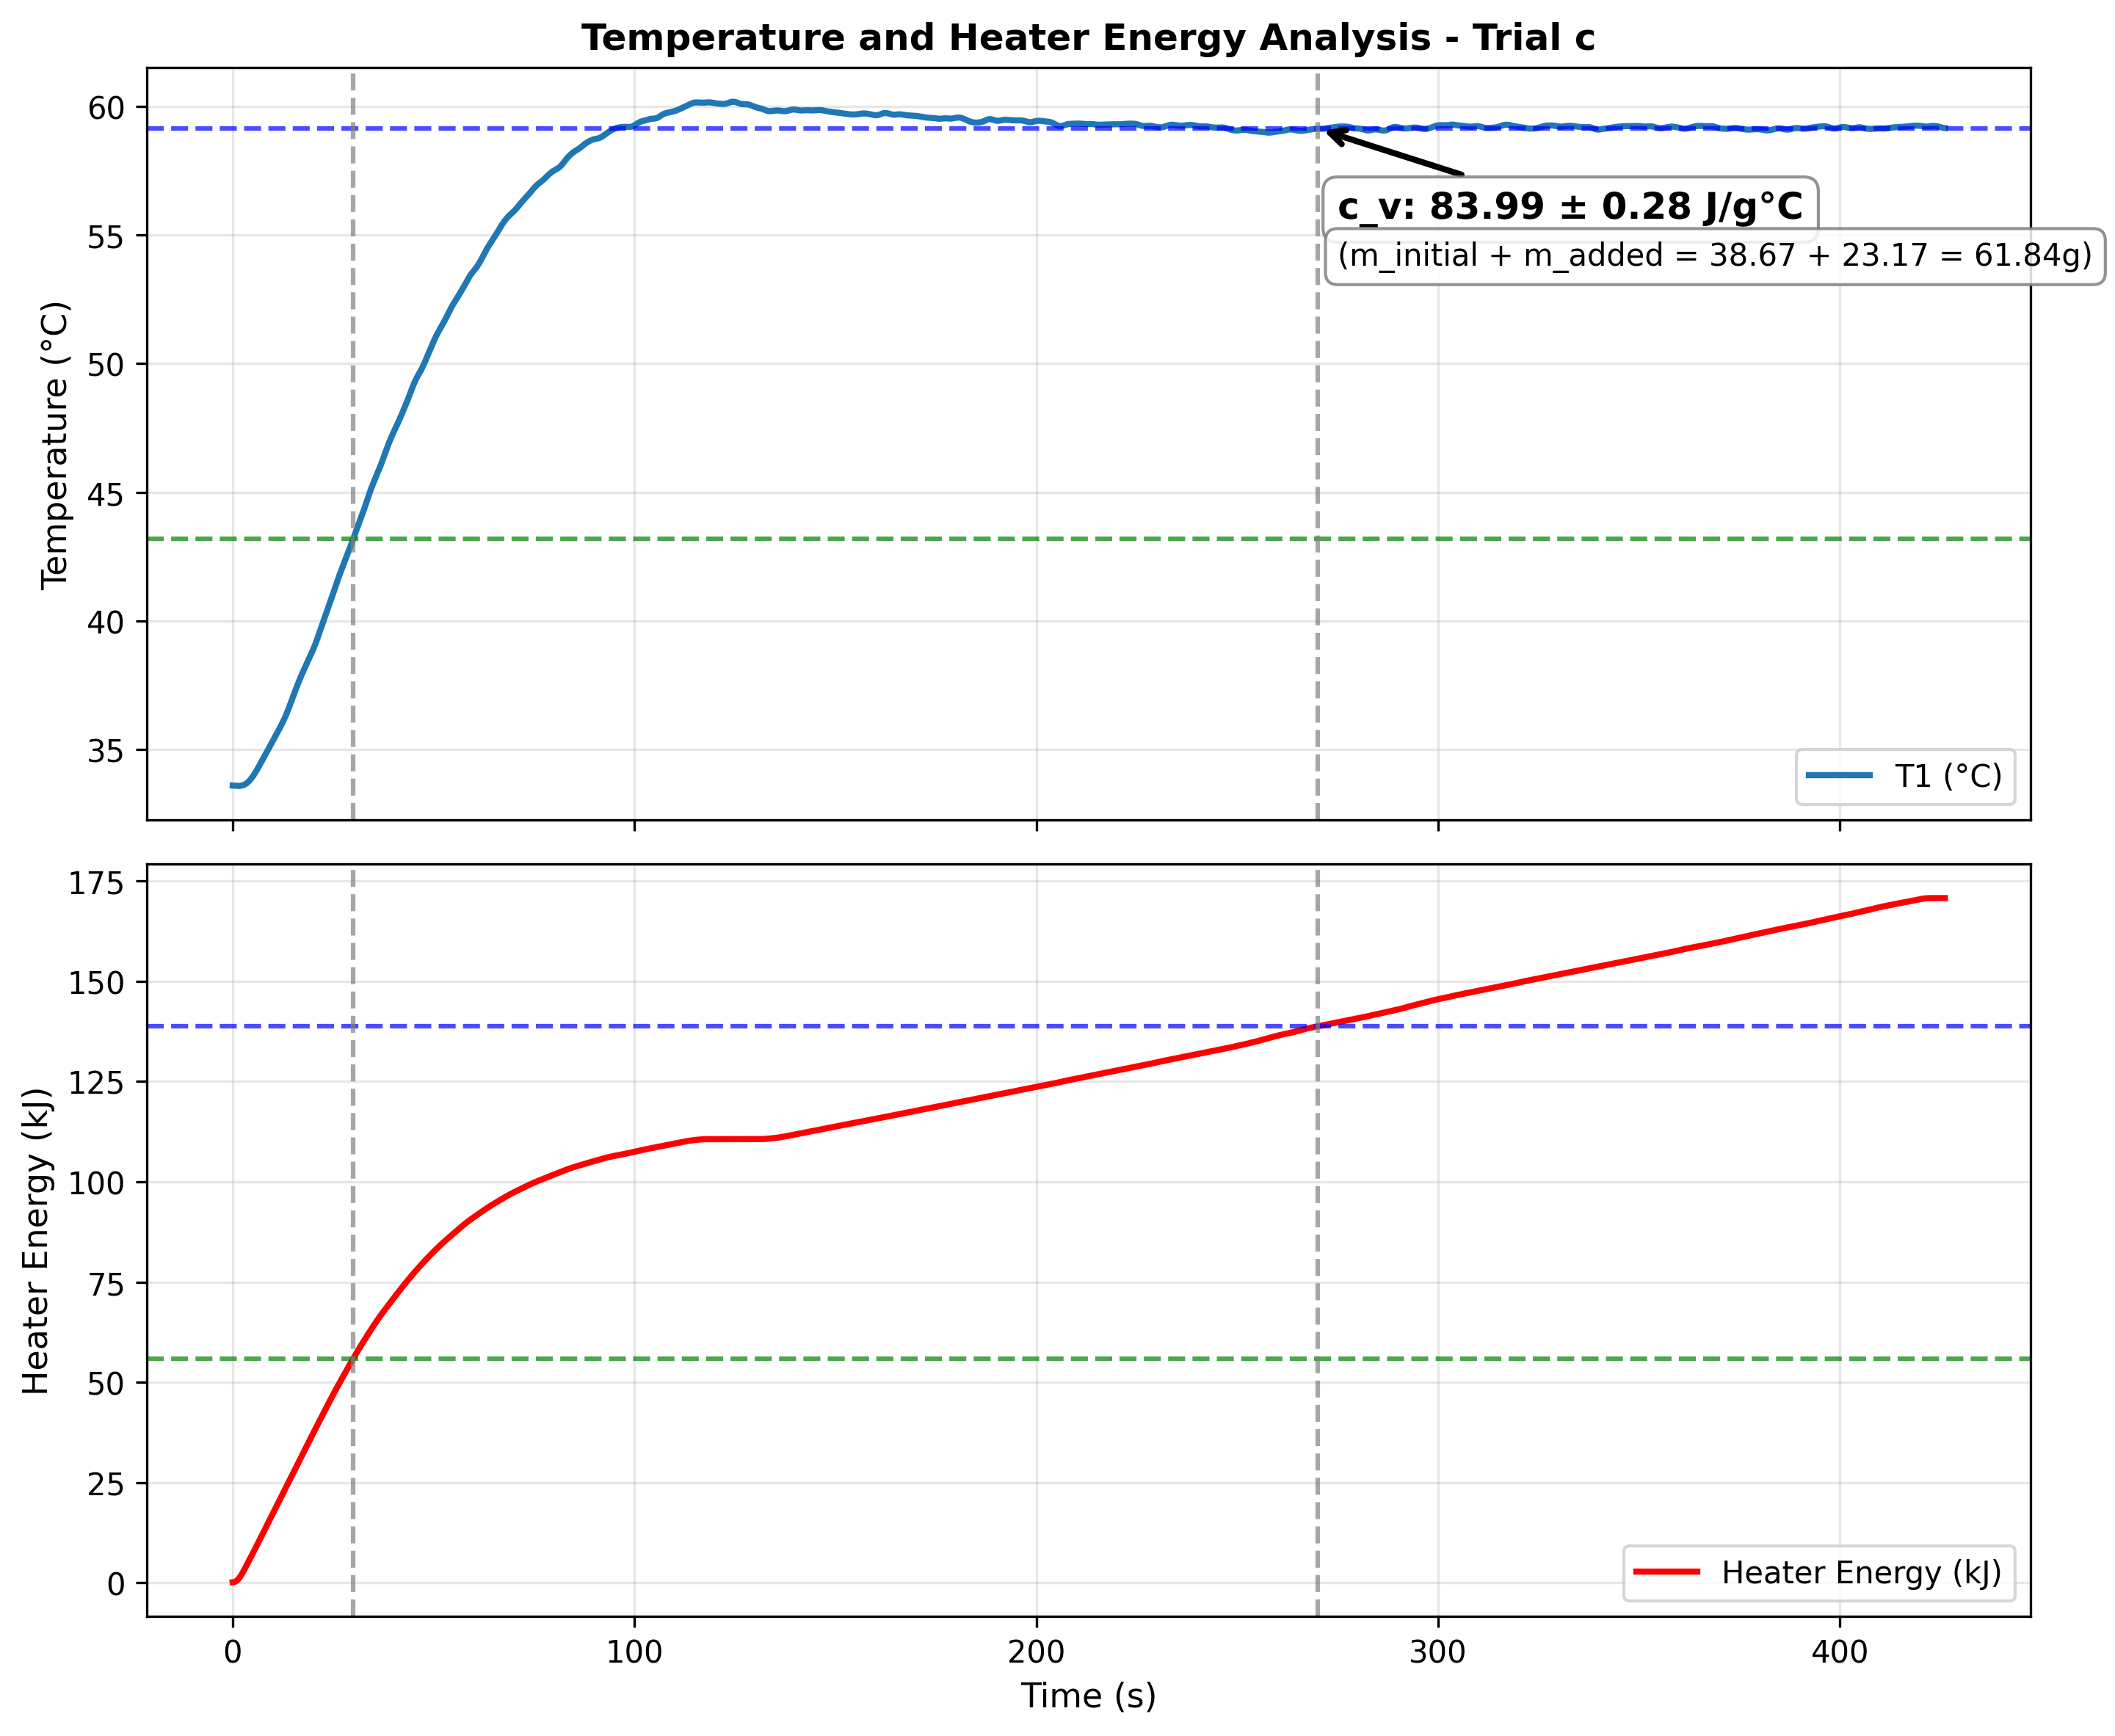
\includegraphics[width=0.30\textwidth]{graphs/part2_trial_c_temp_heater_energy.png}\hfill
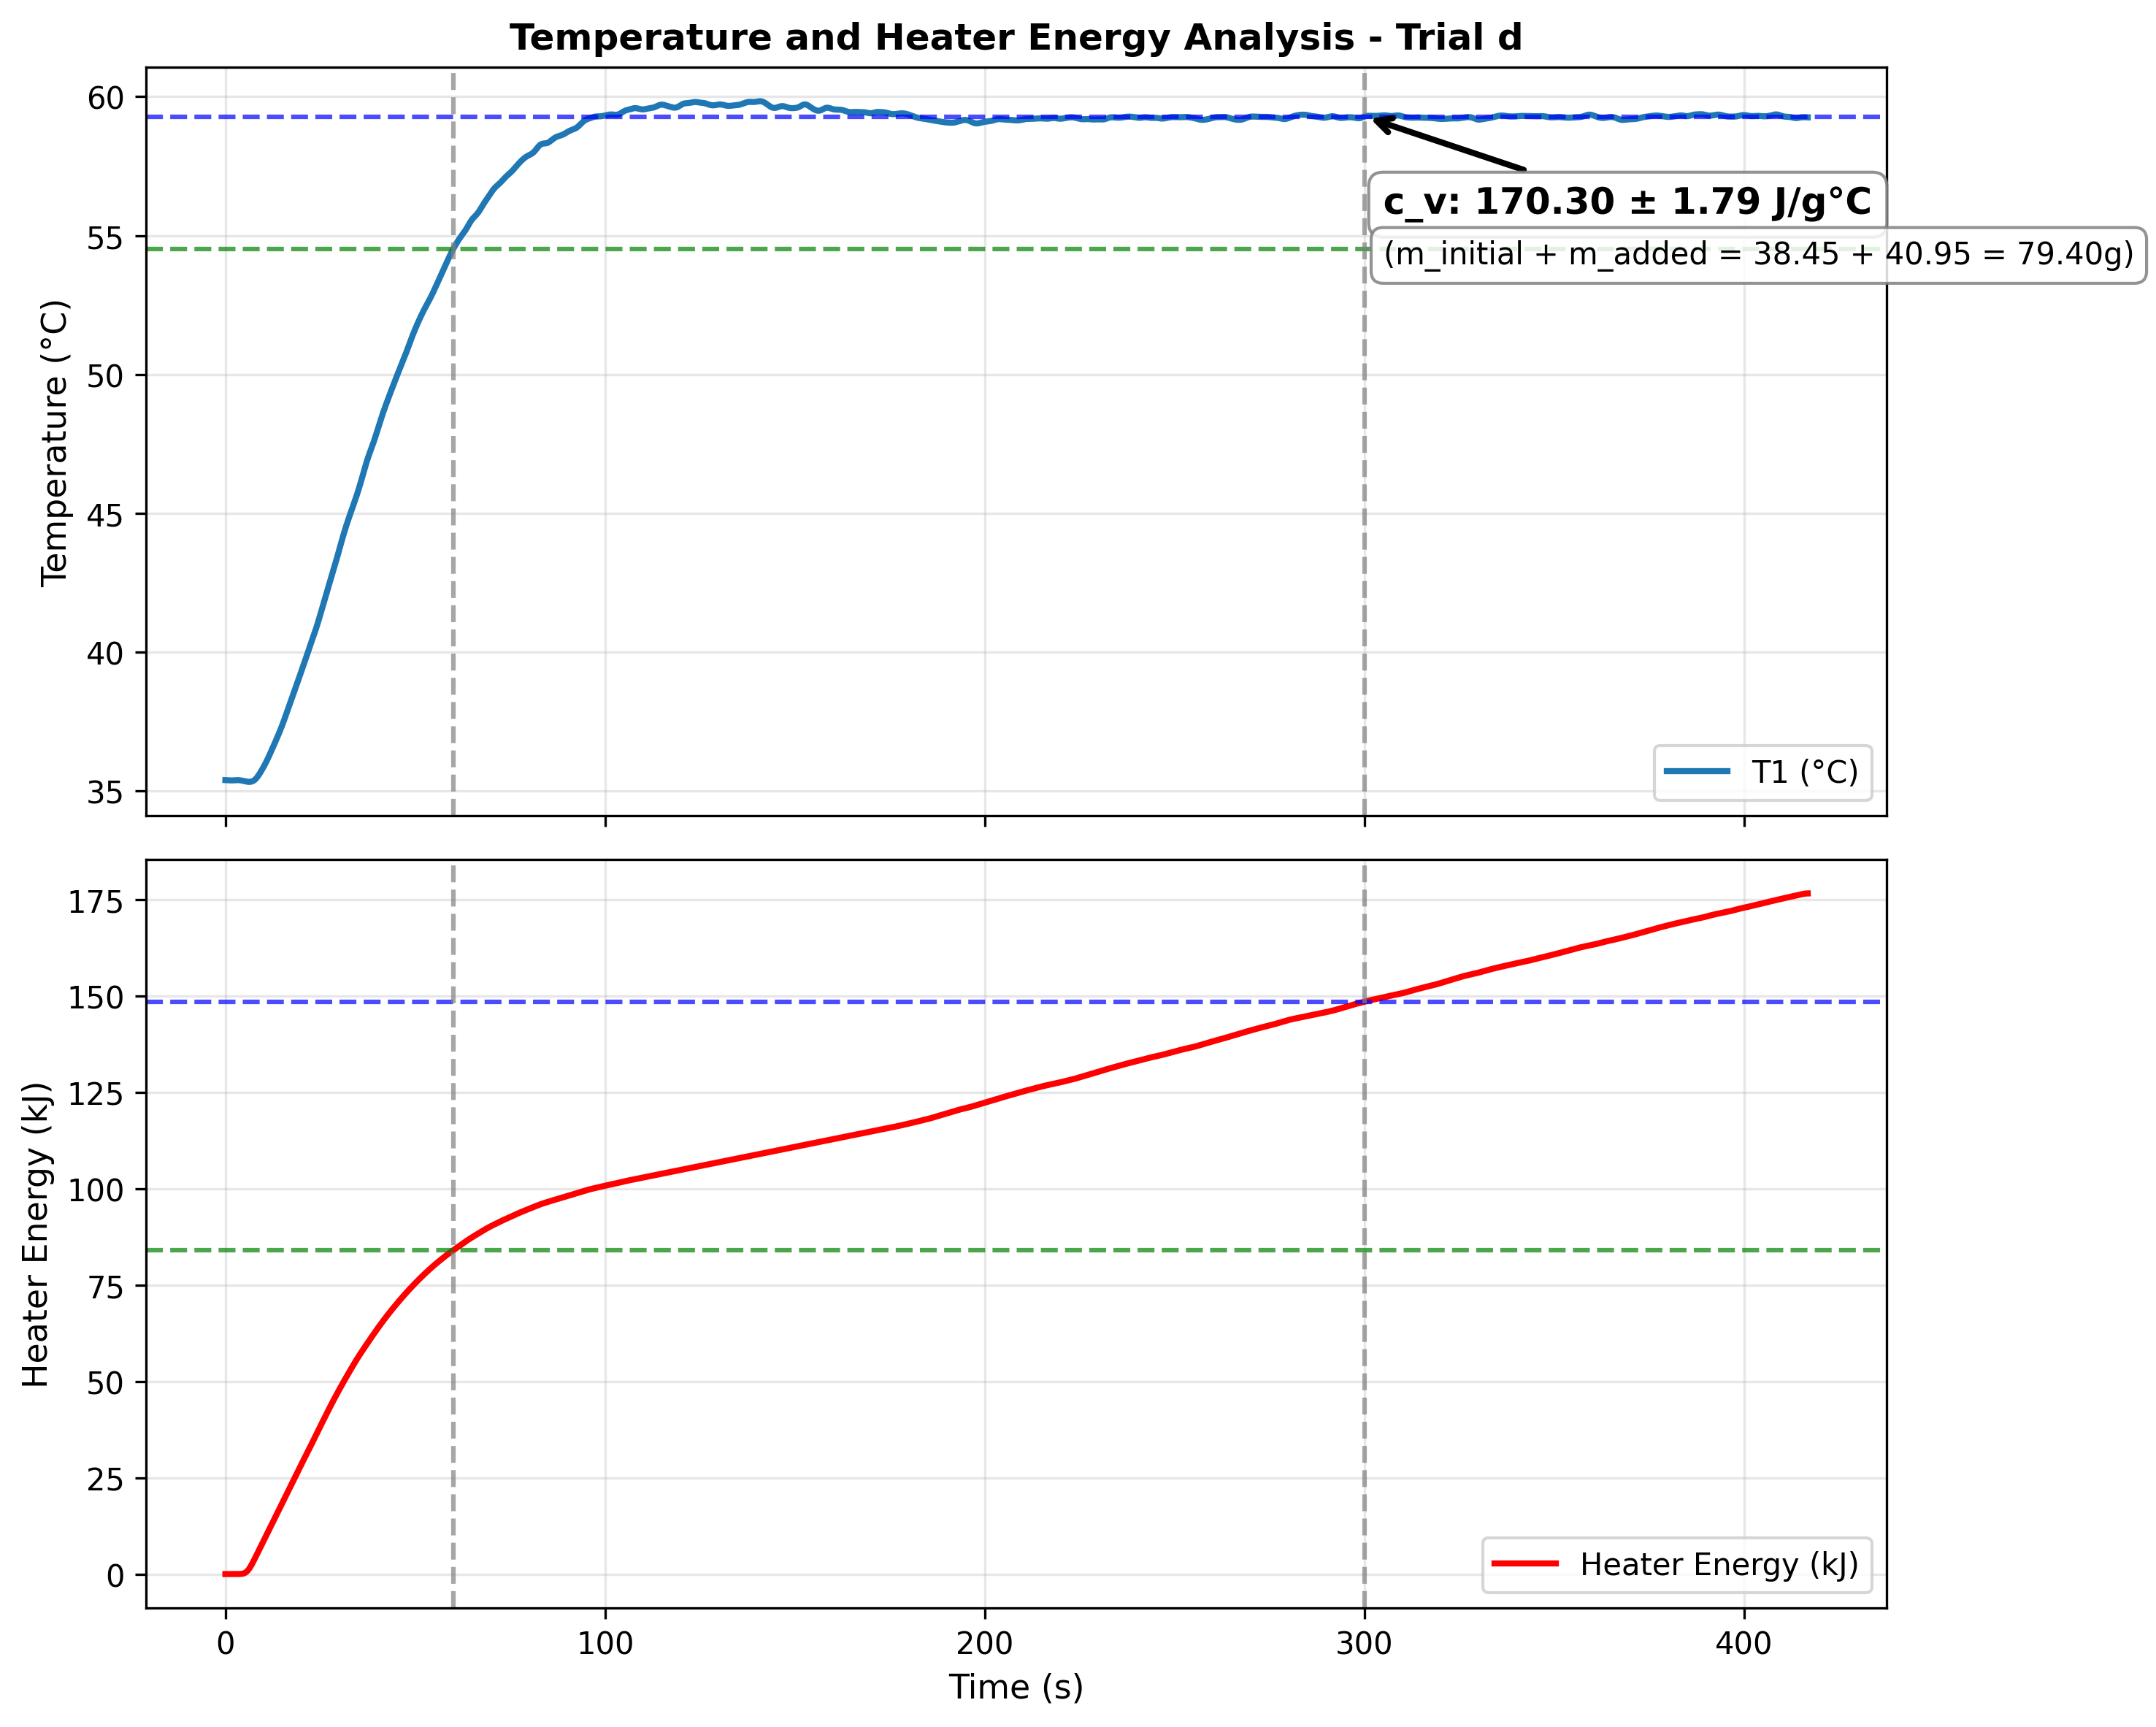
\includegraphics[width=0.30\textwidth]{graphs/part2_trial_d_temp_heater_energy.png}
\caption{Temperature and heater energy: Trials B, C, D (left to right).}
\label{fig:app_temp_energy}
\end{figure}


\subsection*{B.3 Steady-State Maintenance (Trials B, C, D)}

\begin{figure}[H]
\centering
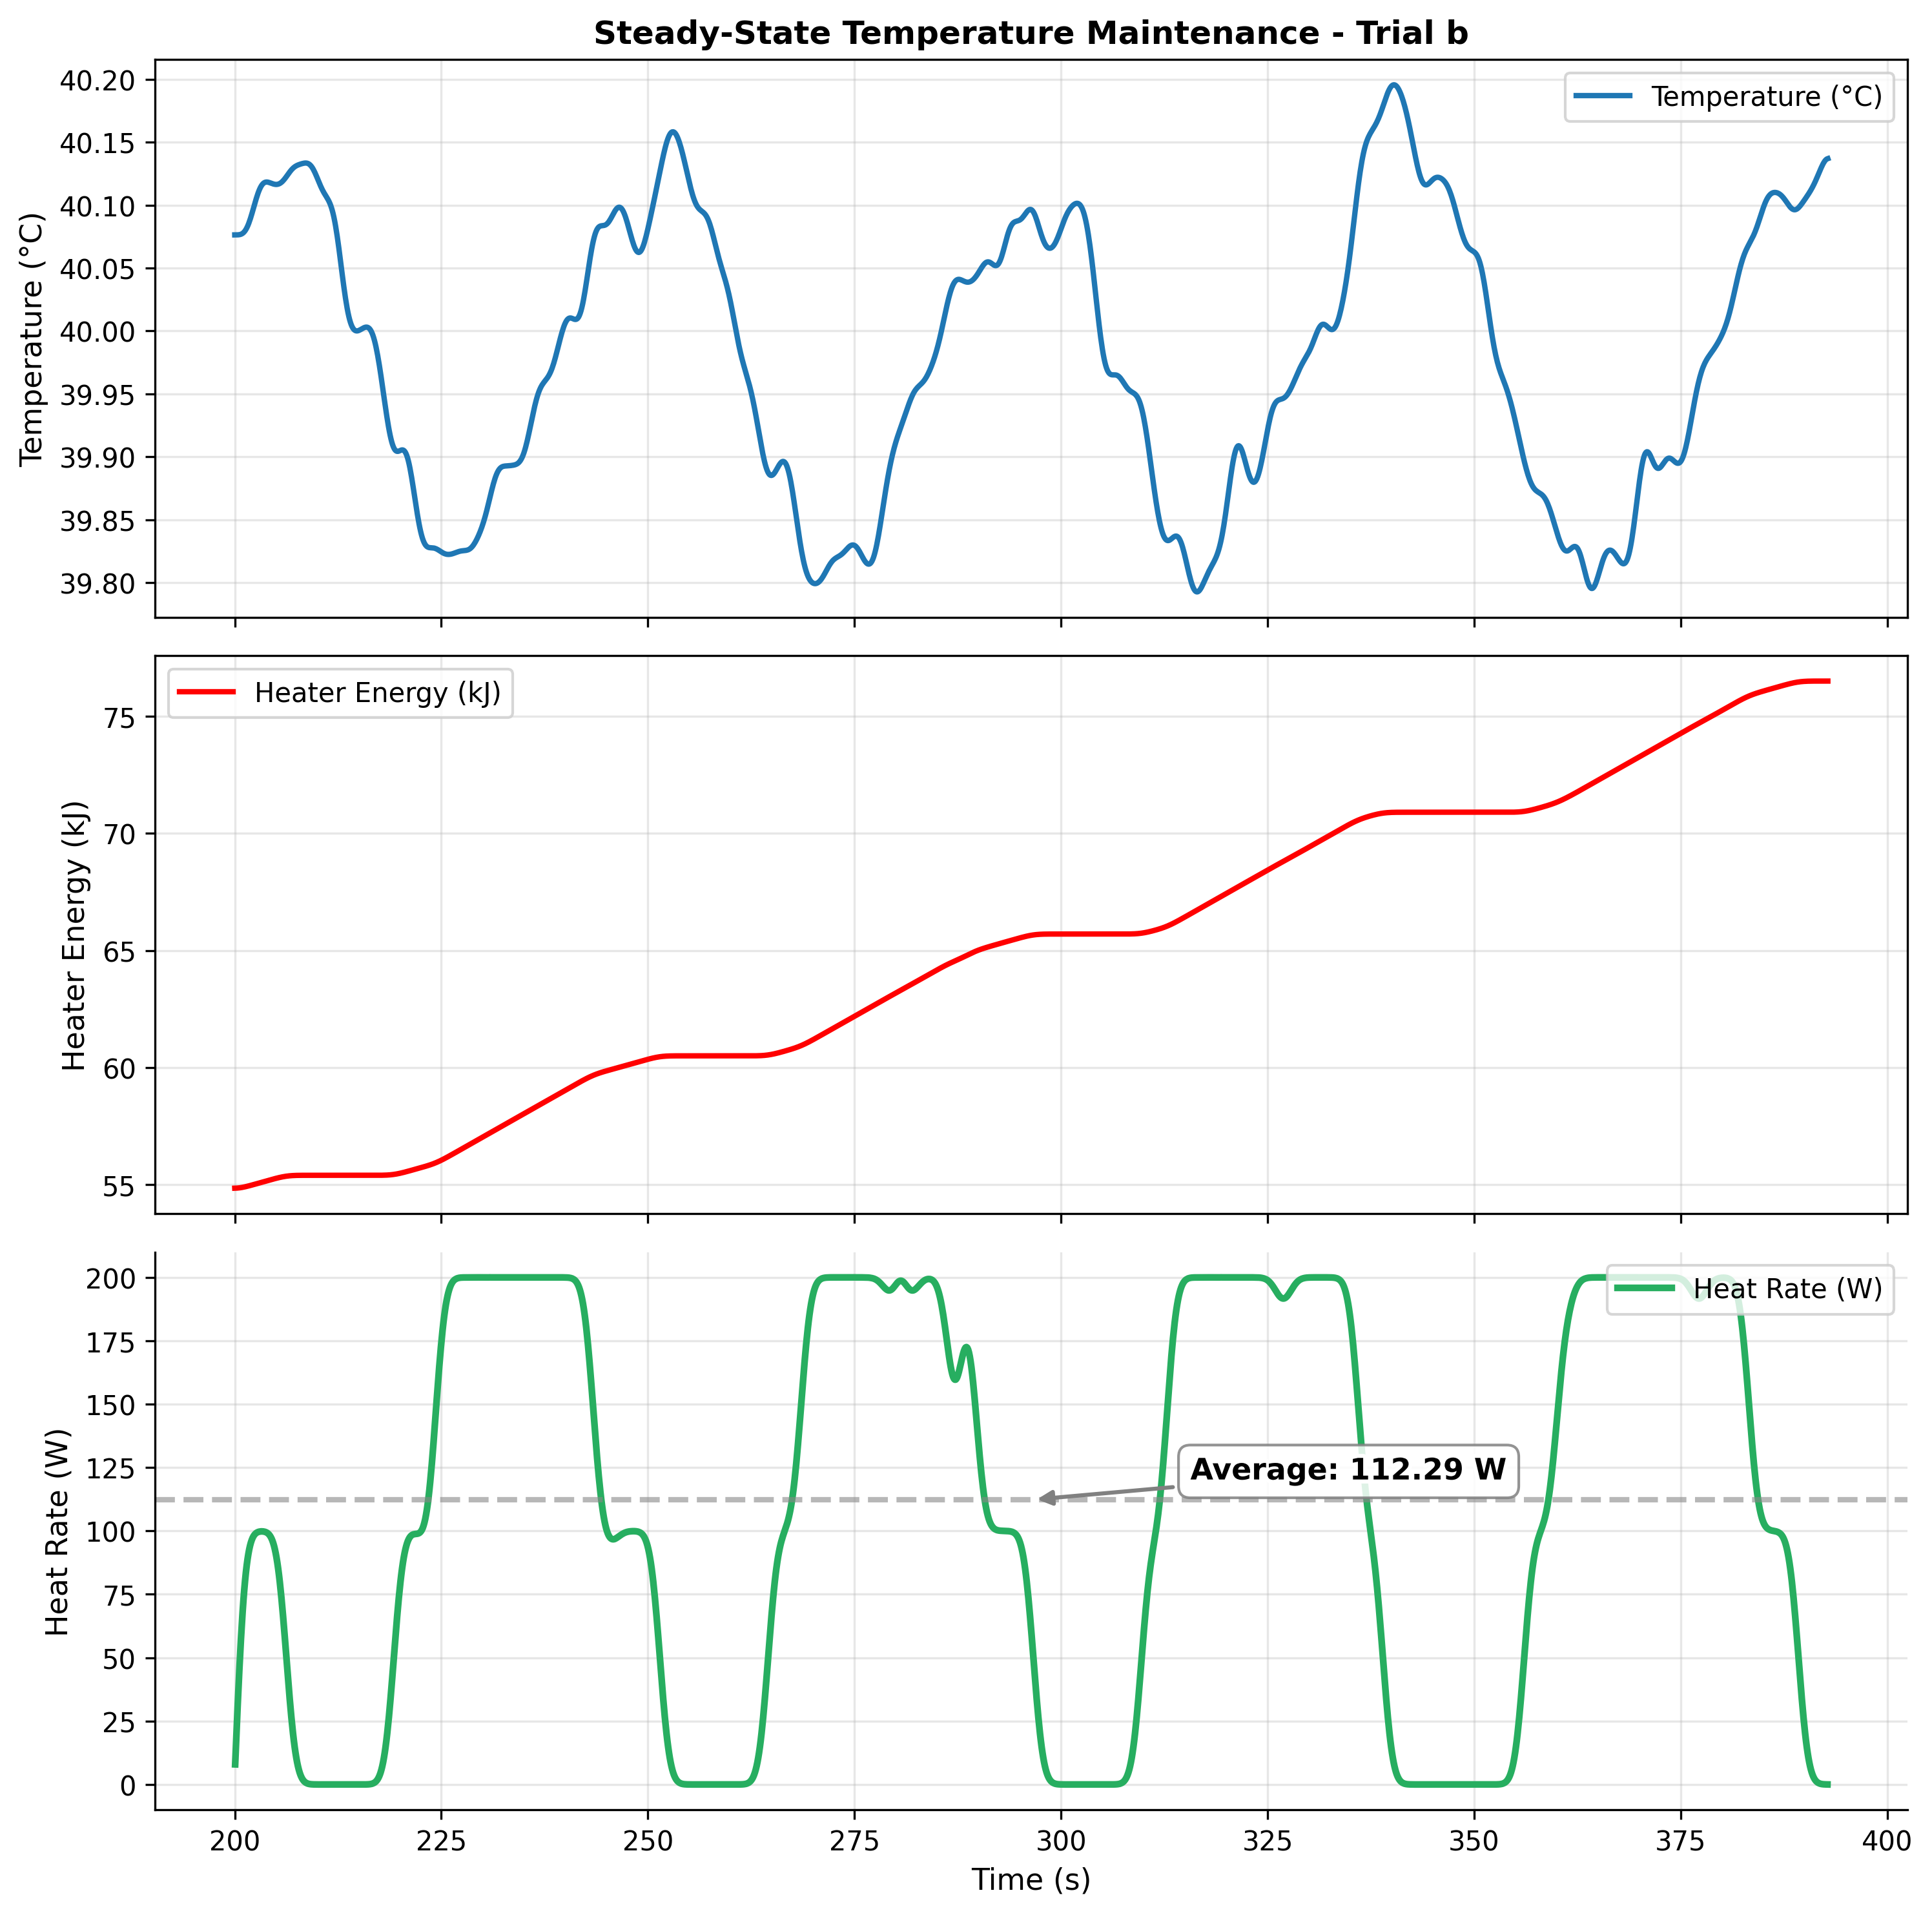
\includegraphics[width=0.30\textwidth]{graphs/part2_trial_b_heater_maintenance.png}\hfill
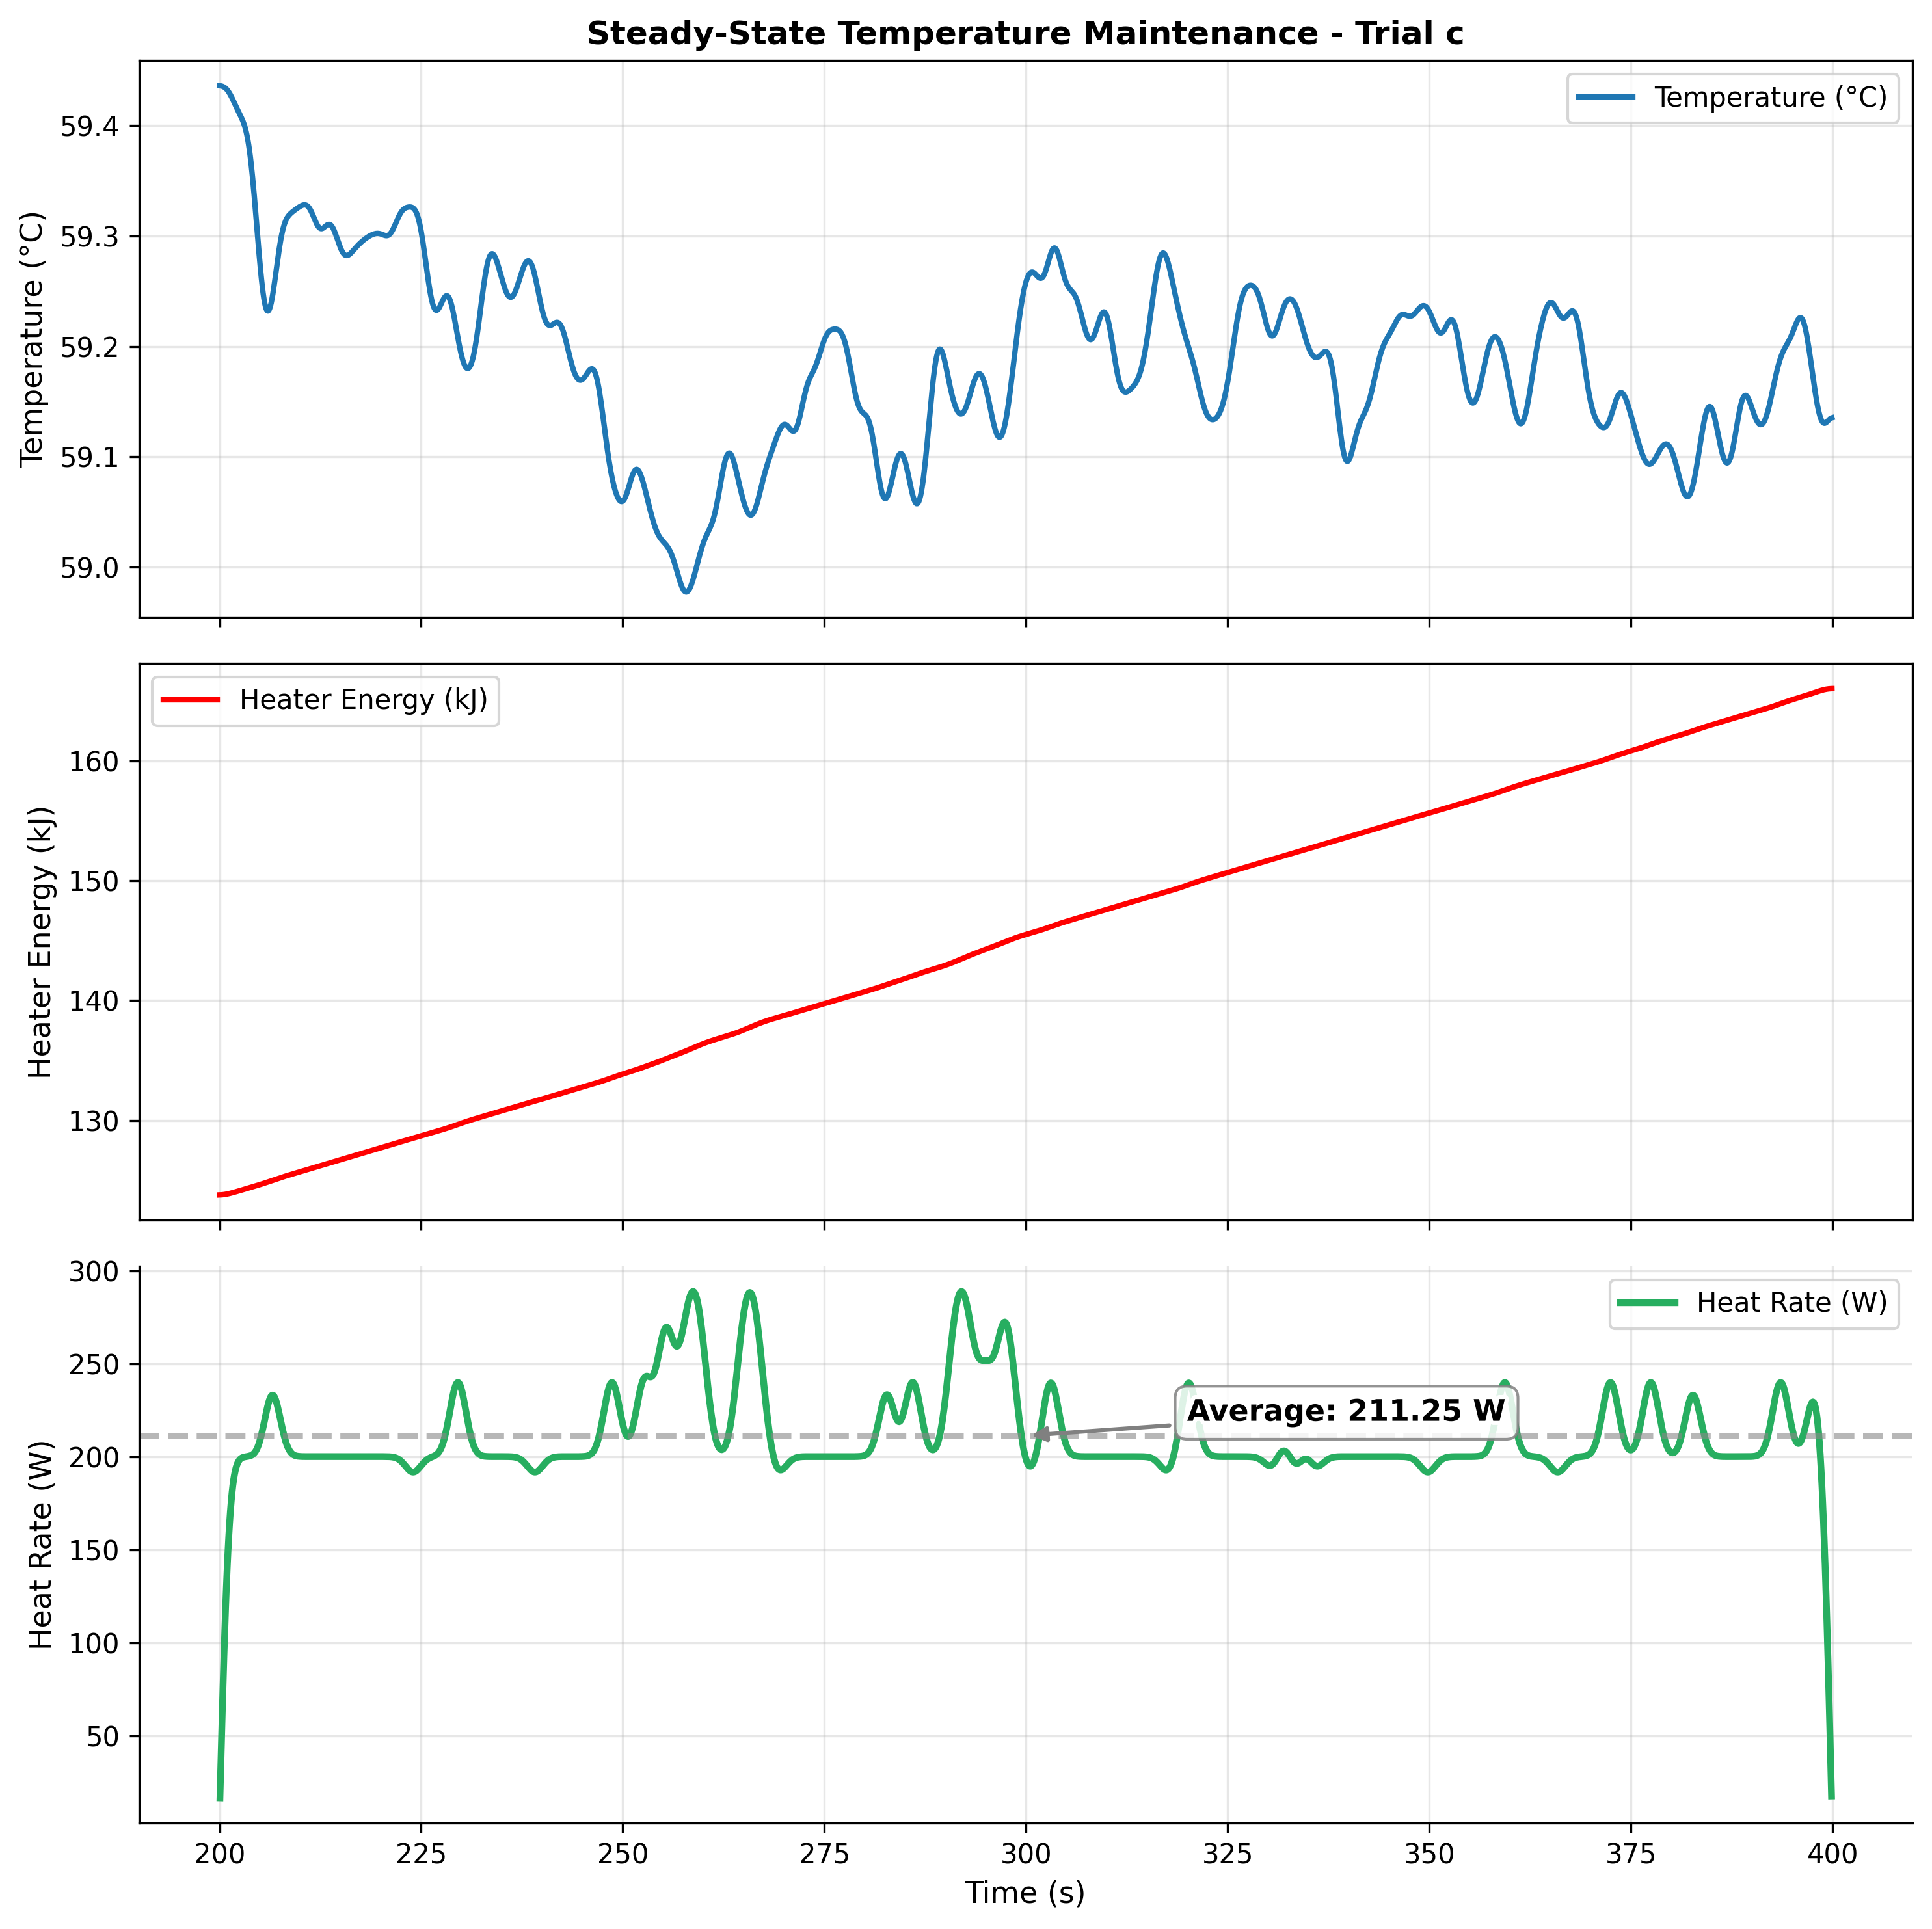
\includegraphics[width=0.30\textwidth]{graphs/part2_trial_c_heater_maintenance.png}\hfill
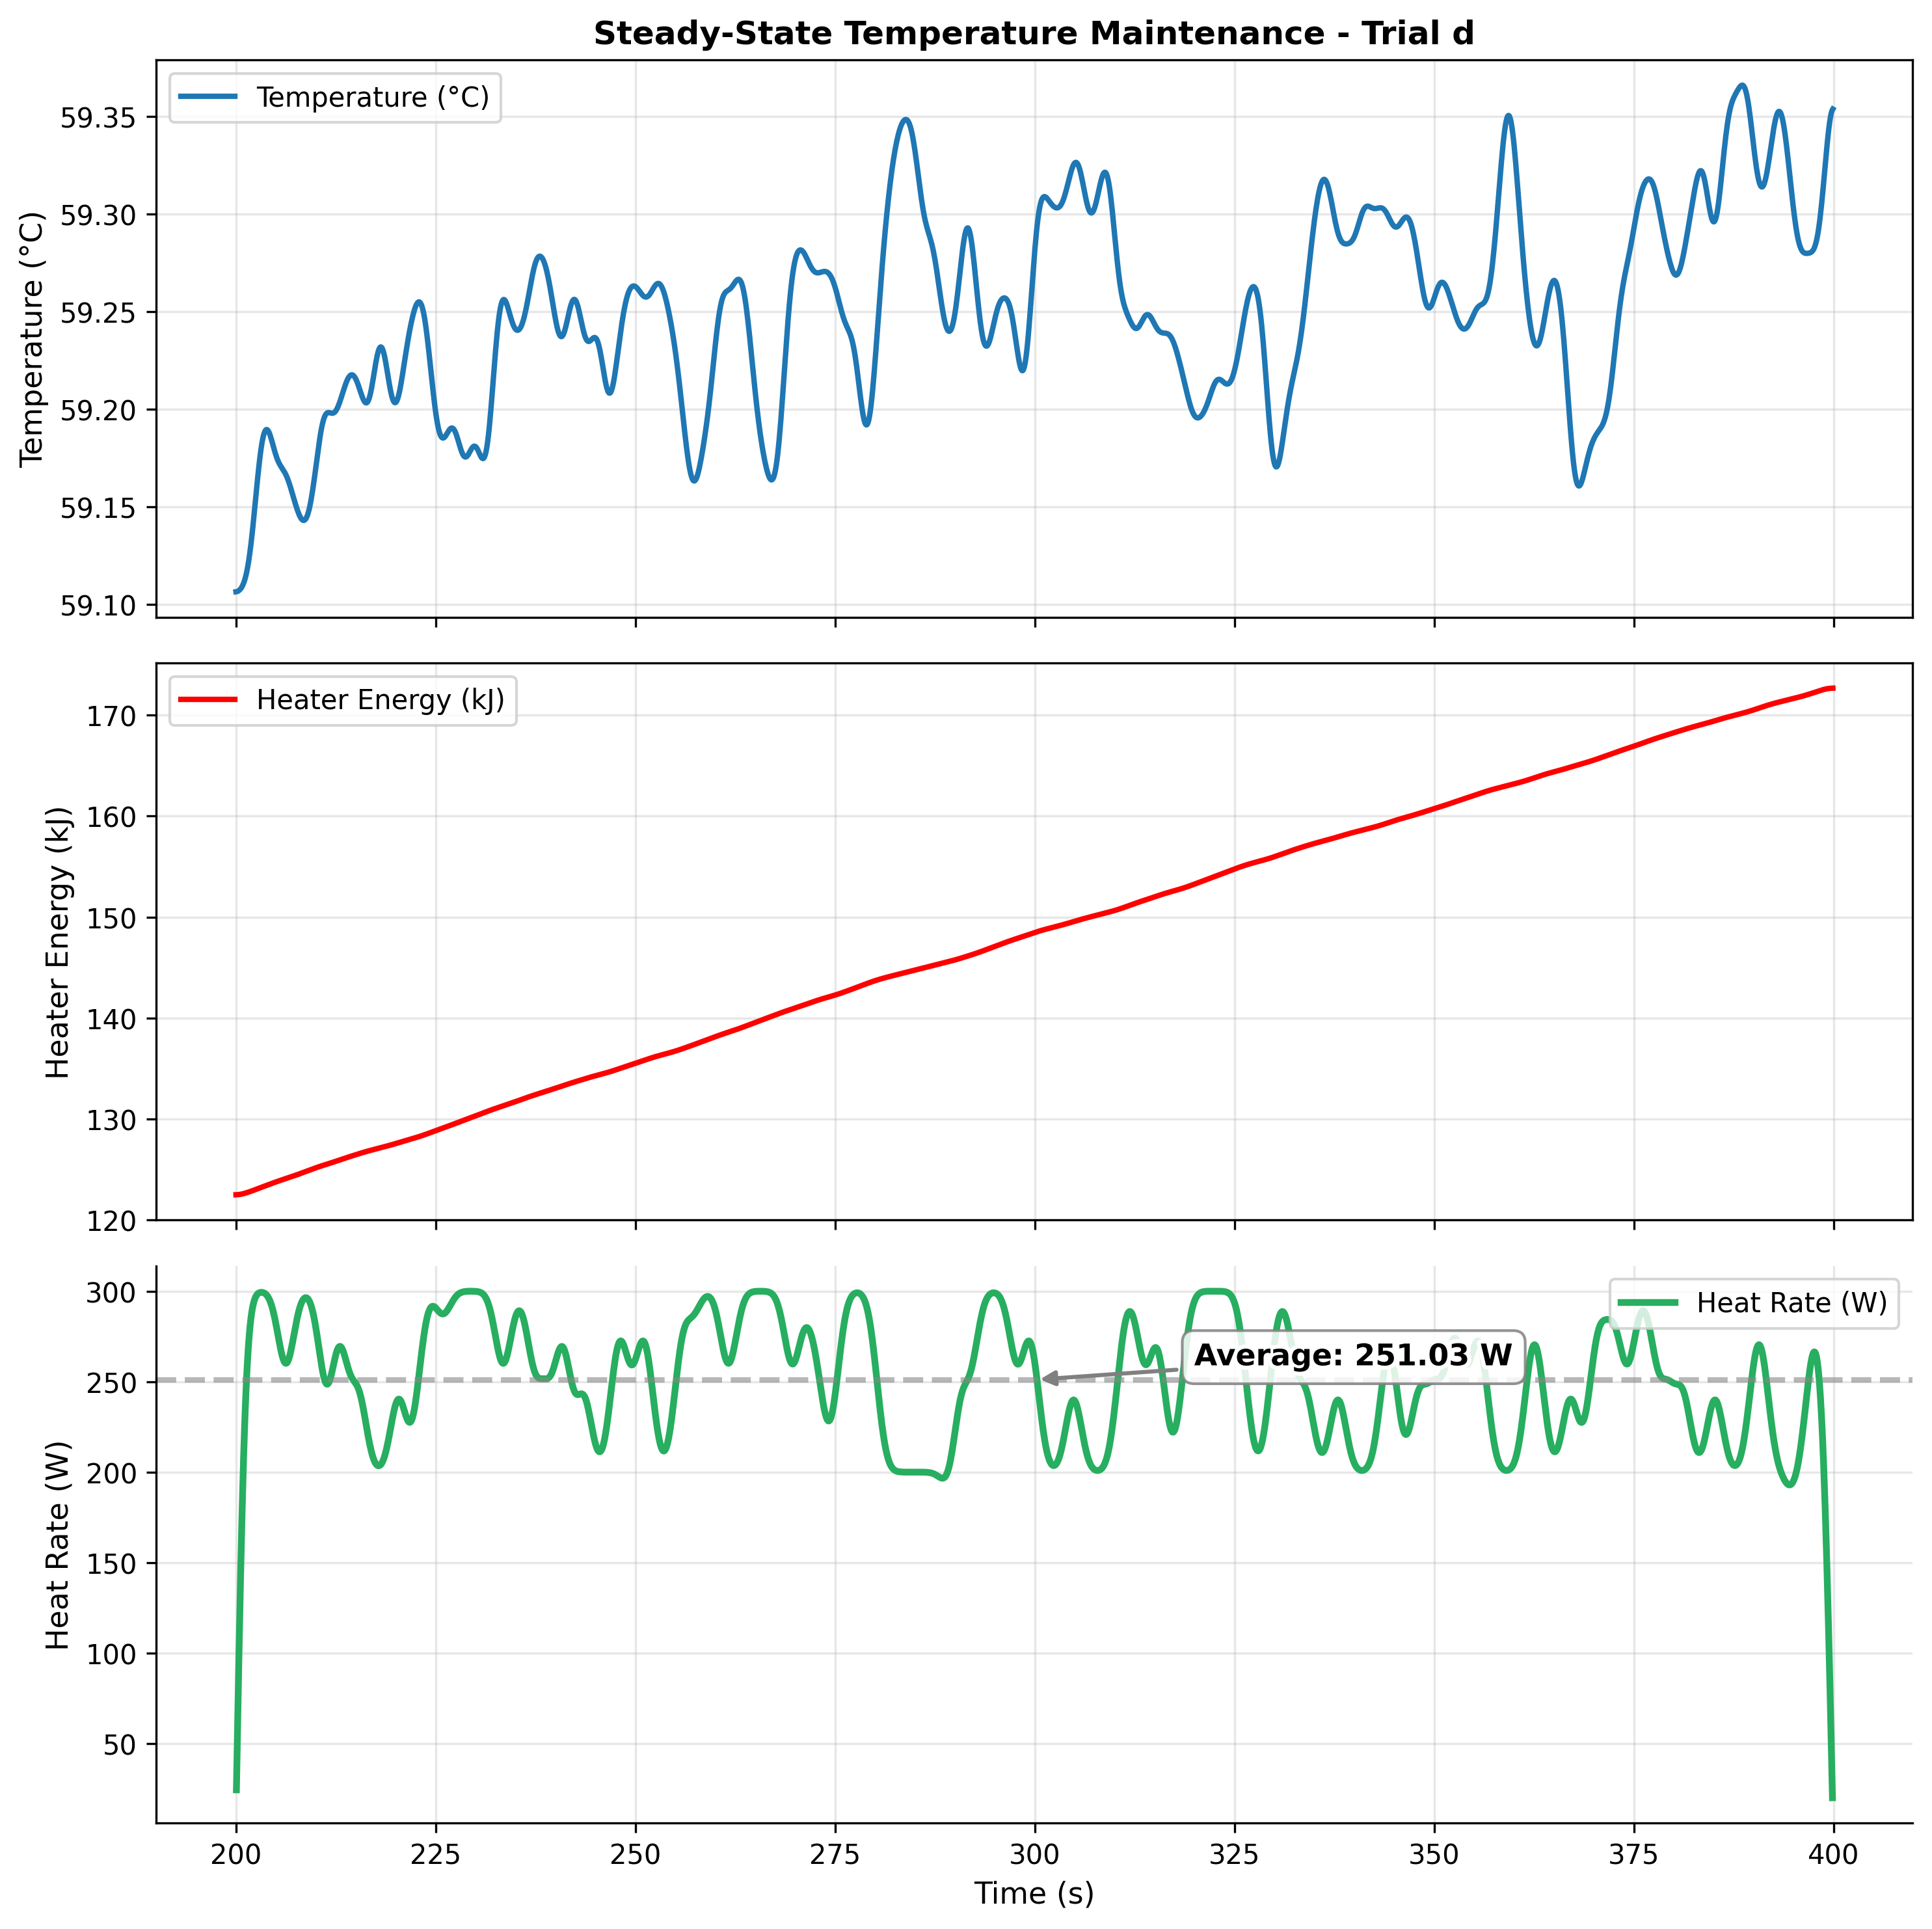
\includegraphics[width=0.30\textwidth]{graphs/part2_trial_d_heater_maintenance.png}
\caption{Steady-state plateau:Trials B, C, D (left to right).}
\label{fig:app_maintenance}
\end{figure}

\subsection*{B.4 Heat Loss Breakdown (Trials B, C, D)}

\begin{figure}[H]
\centering
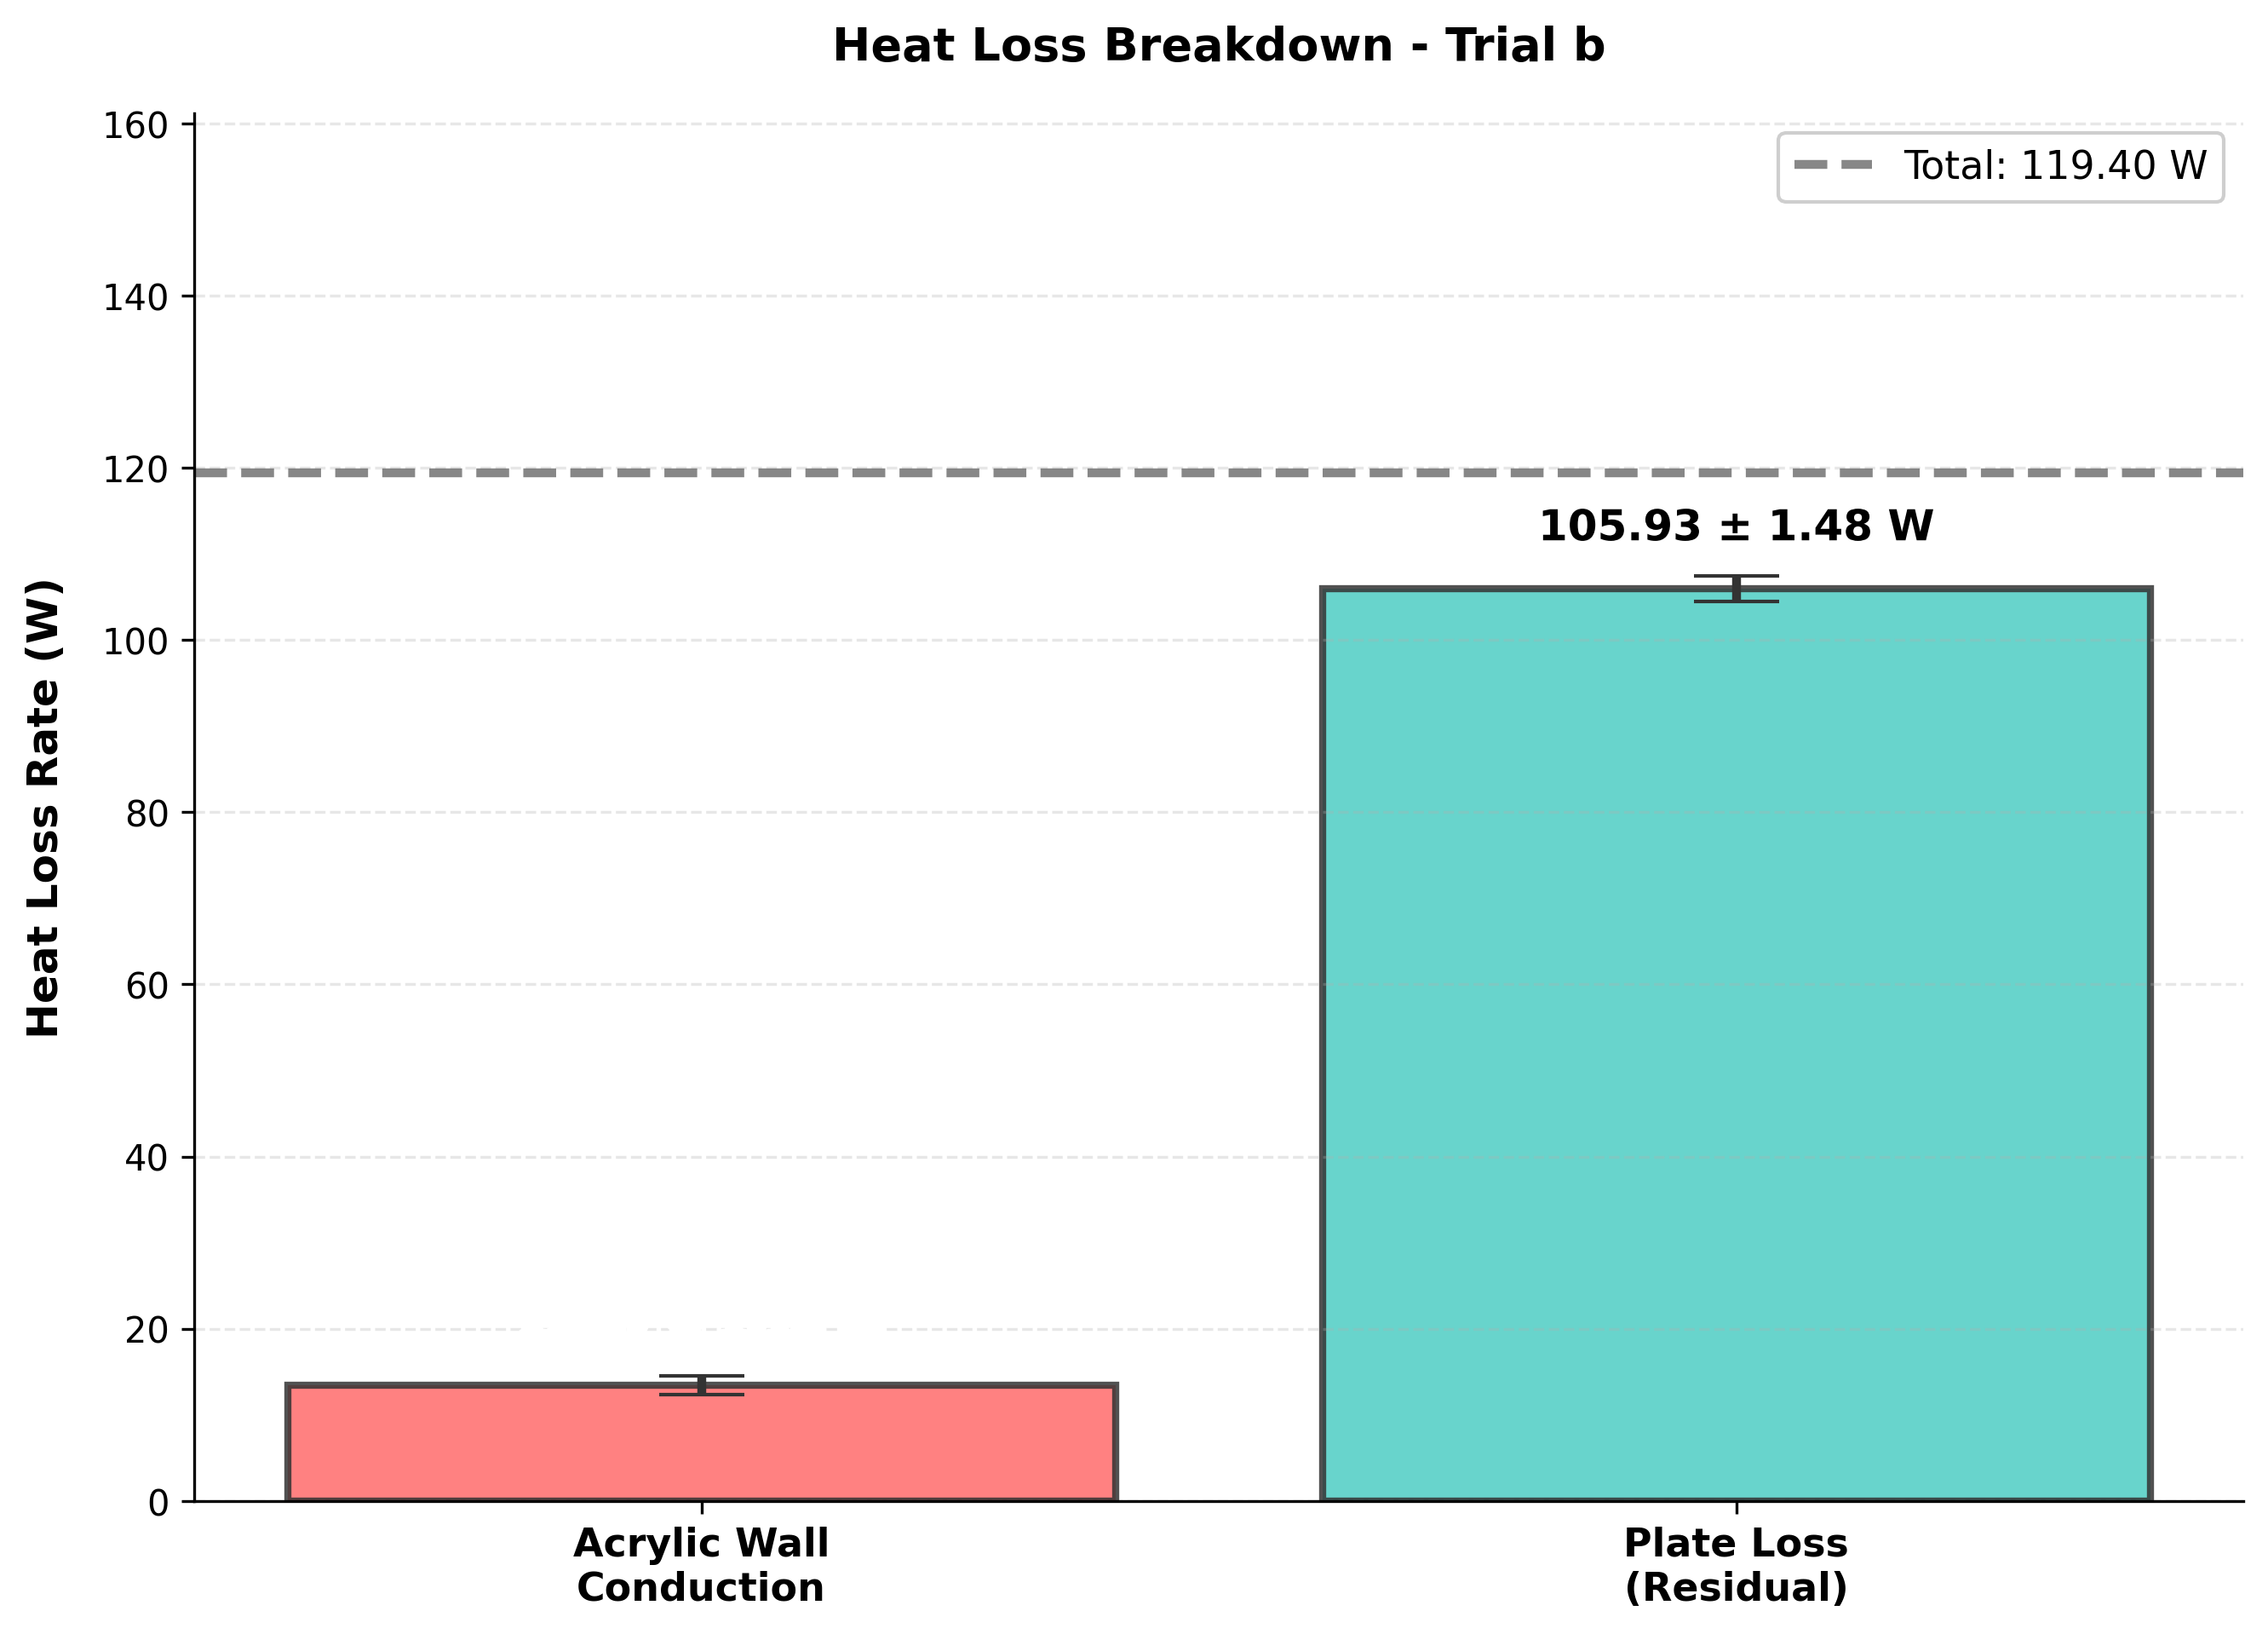
\includegraphics[width=0.28\textwidth]{graphs/part2_trial_b_loss_breakdown.png}\hfill
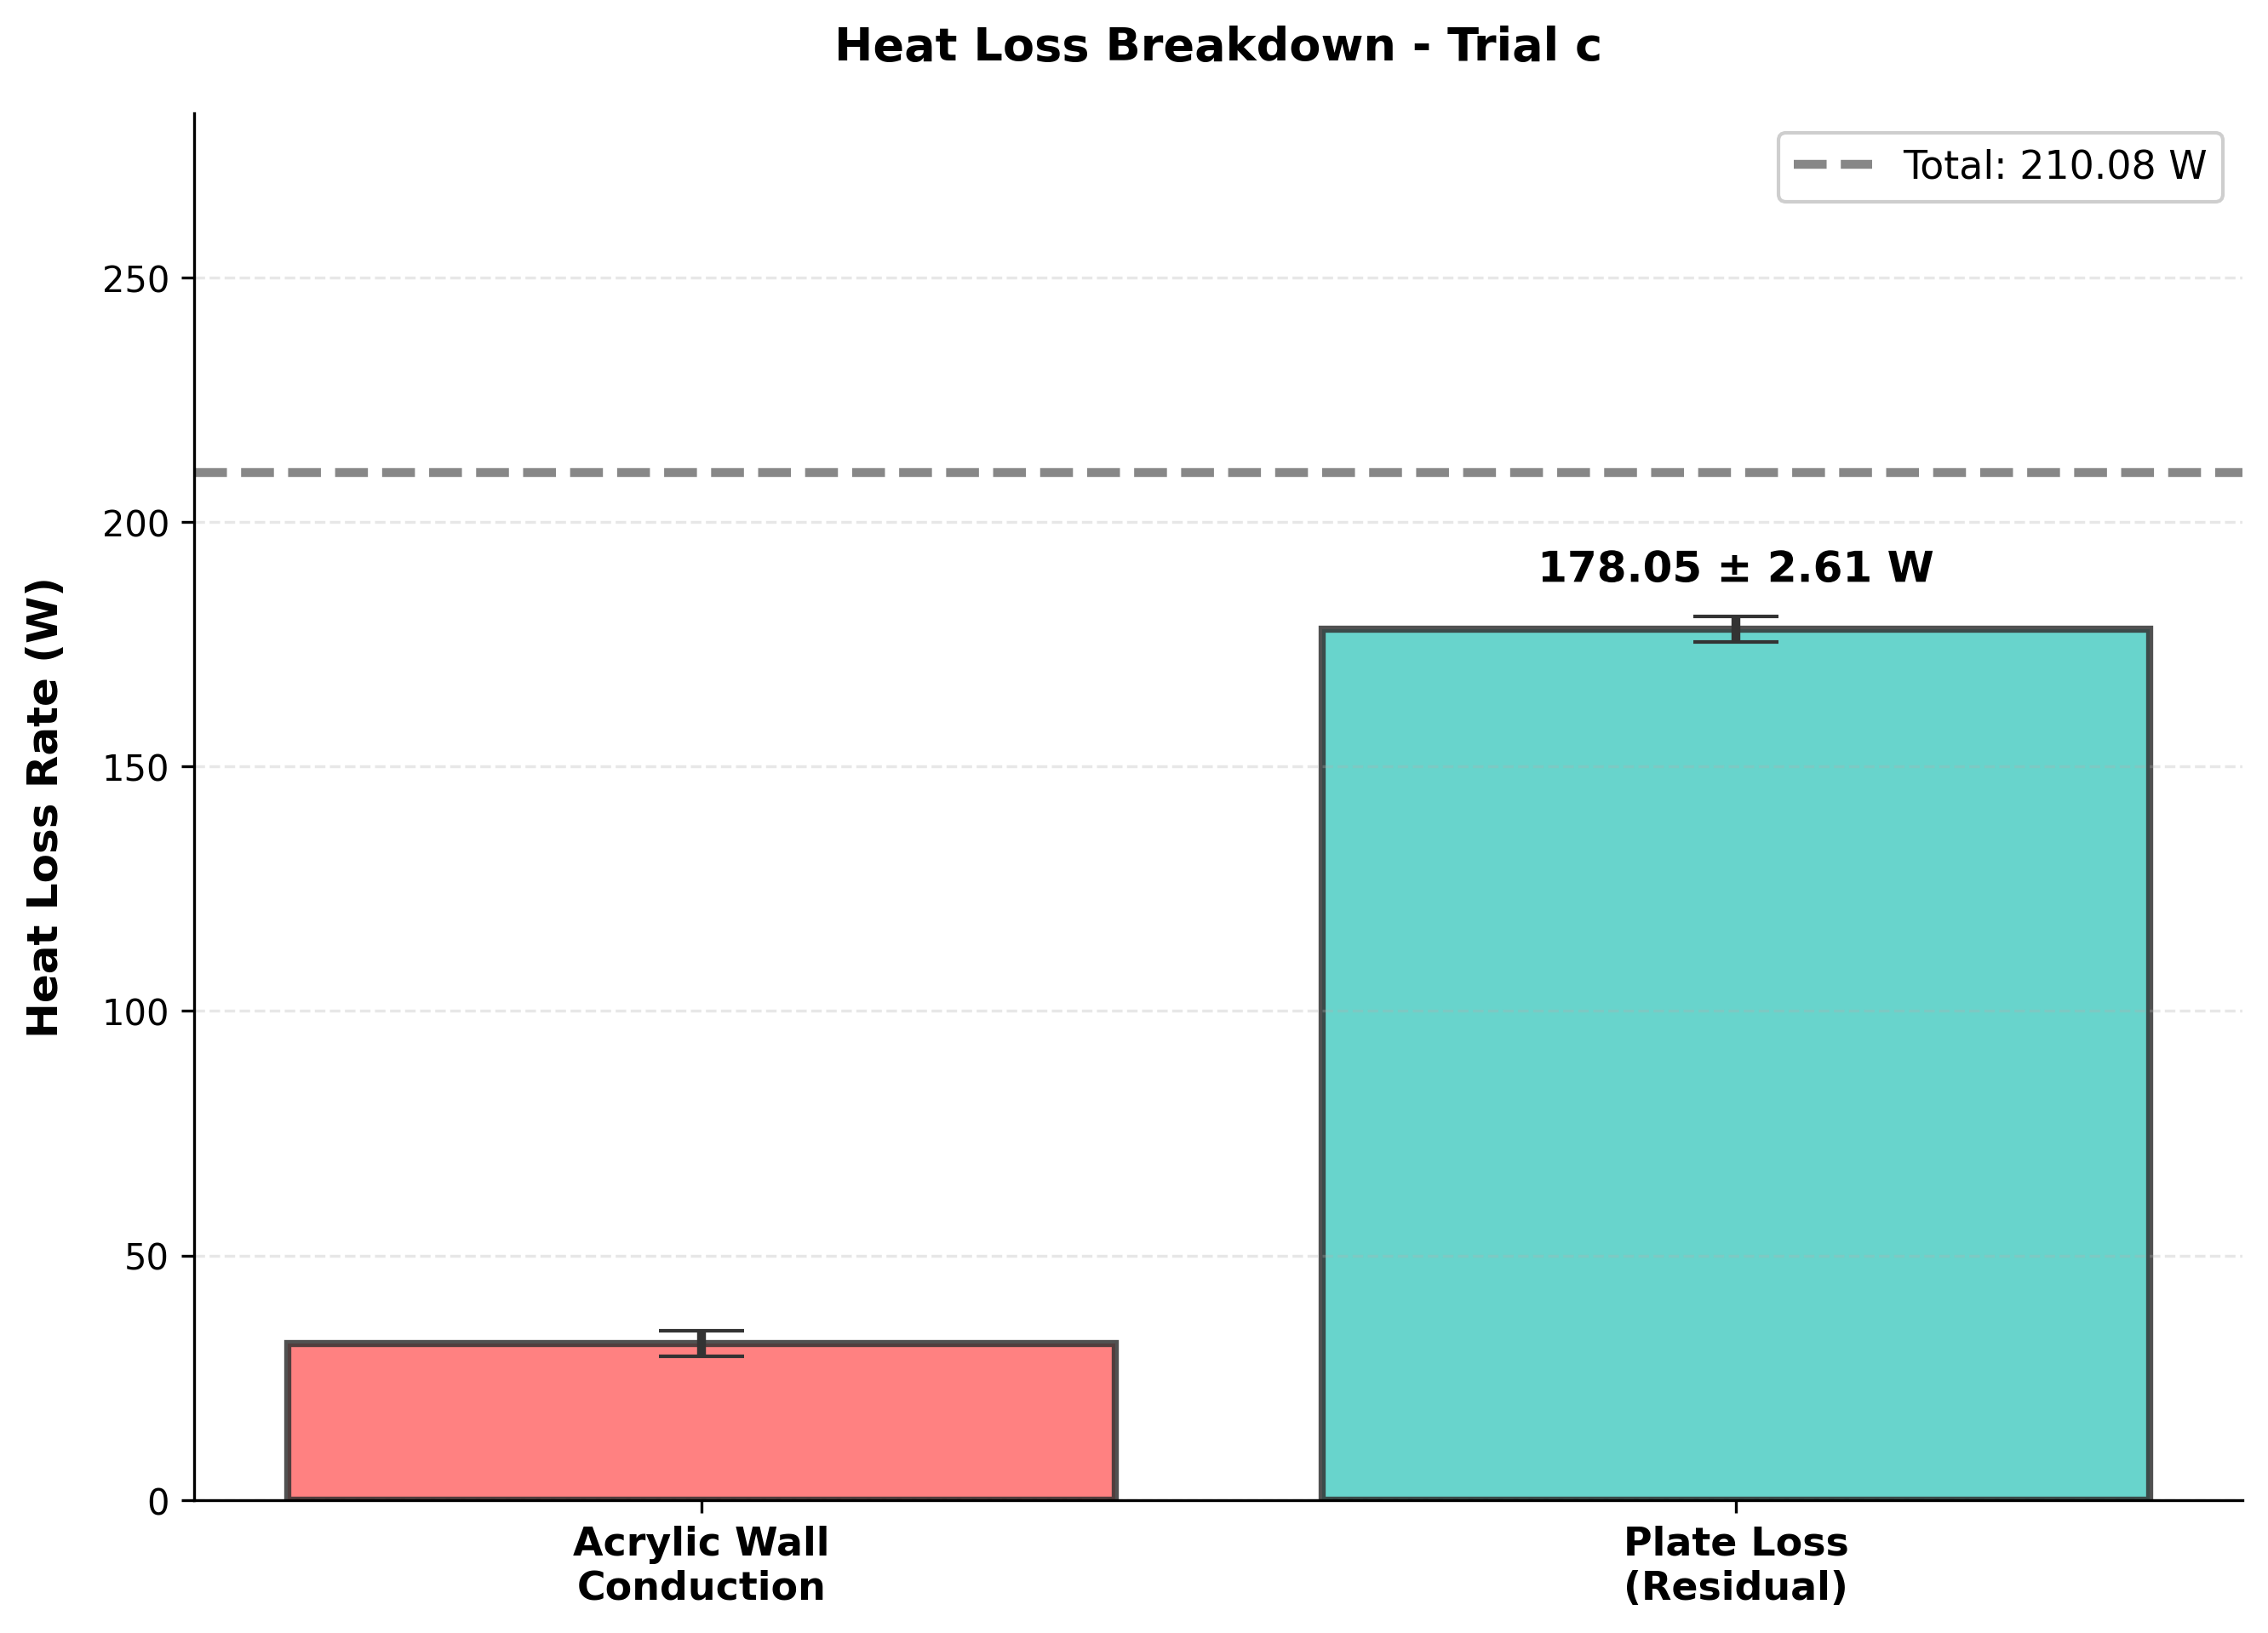
\includegraphics[width=0.28\textwidth]{graphs/part2_trial_c_loss_breakdown.png}\hfill
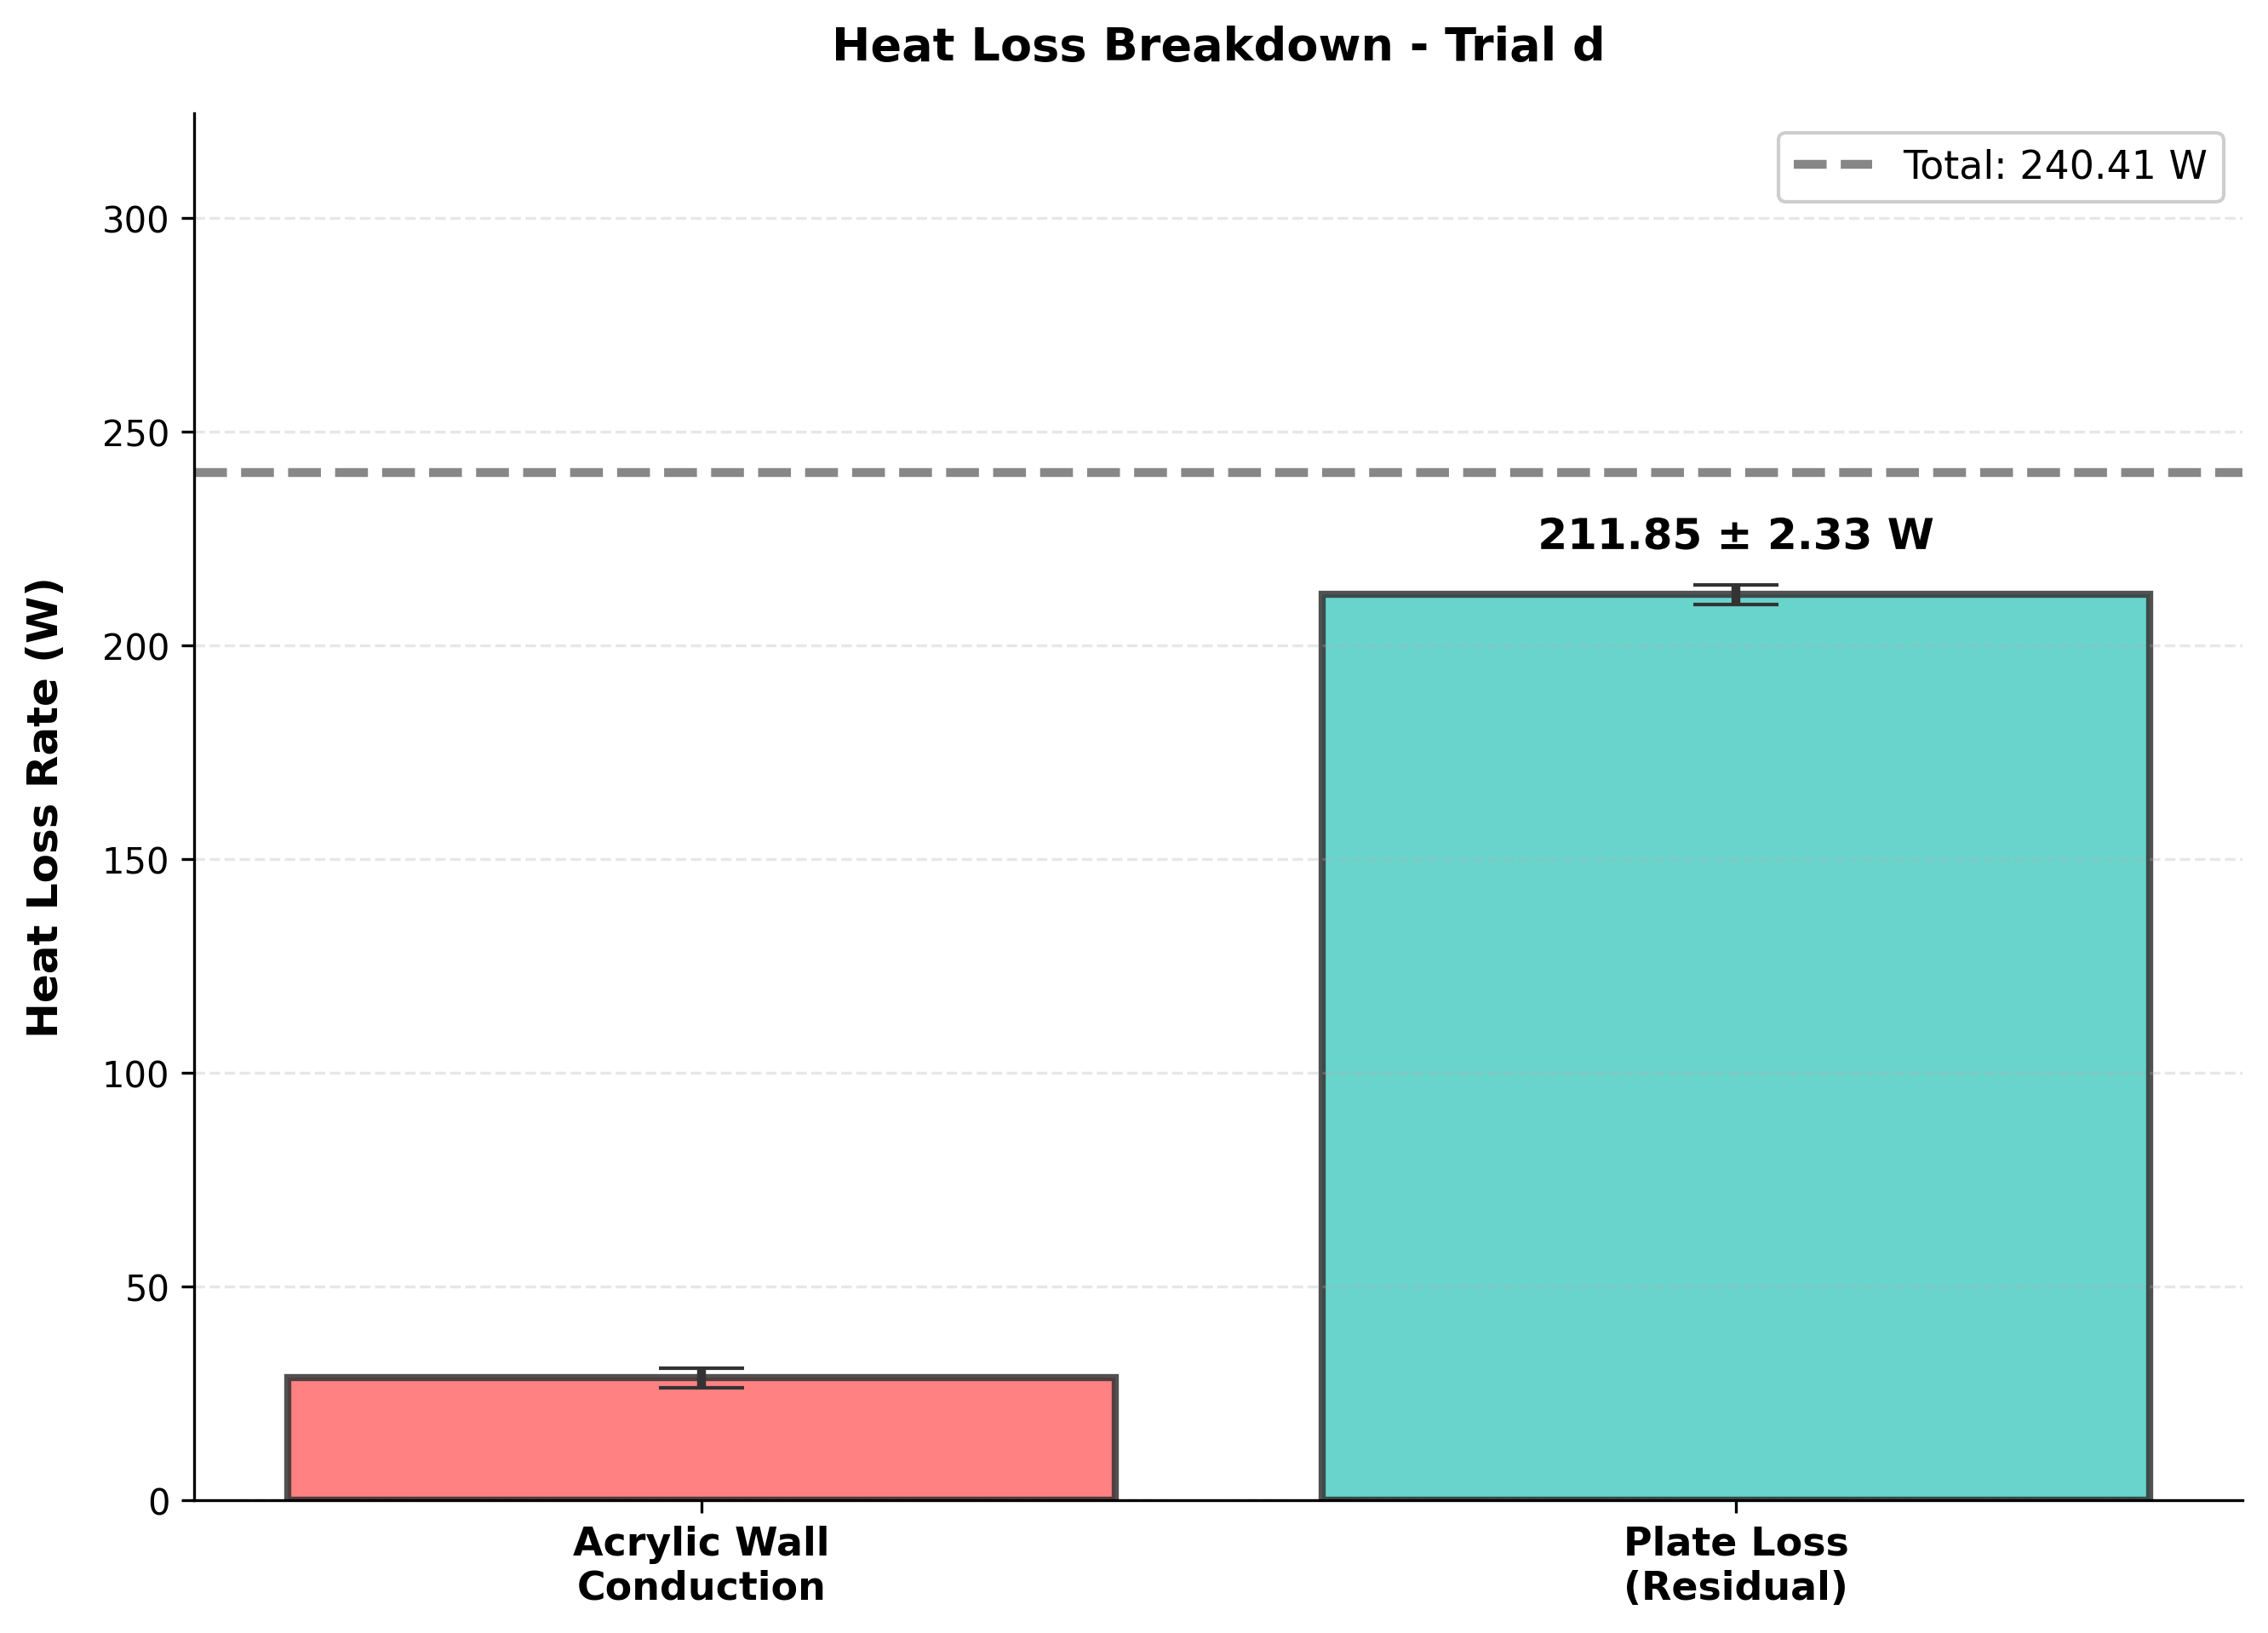
\includegraphics[width=0.28\textwidth]{graphs/part2_trial_d_loss_breakdown.png}
\caption{Heat loss breakdown (wall vs.\ plate): Trials B, C, D (left to right).}
\label{fig:app_breakdown}
\end{figure}

\end{document}
